% Options for packages loaded elsewhere
\PassOptionsToPackage{unicode}{hyperref}
\PassOptionsToPackage{hyphens}{url}
\PassOptionsToPackage{dvipsnames,svgnames*,x11names*}{xcolor}
%
\documentclass[
  12pt,
]{book}
\usepackage{lmodern}
\usepackage{amssymb,amsmath}
\usepackage{ifxetex,ifluatex}
\ifnum 0\ifxetex 1\fi\ifluatex 1\fi=0 % if pdftex
  \usepackage[T1]{fontenc}
  \usepackage[utf8]{inputenc}
  \usepackage{textcomp} % provide euro and other symbols
\else % if luatex or xetex
  \usepackage{unicode-math}
  \defaultfontfeatures{Scale=MatchLowercase}
  \defaultfontfeatures[\rmfamily]{Ligatures=TeX,Scale=1}
\fi
% Use upquote if available, for straight quotes in verbatim environments
\IfFileExists{upquote.sty}{\usepackage{upquote}}{}
\IfFileExists{microtype.sty}{% use microtype if available
  \usepackage[]{microtype}
  \UseMicrotypeSet[protrusion]{basicmath} % disable protrusion for tt fonts
}{}
\makeatletter
\@ifundefined{KOMAClassName}{% if non-KOMA class
  \IfFileExists{parskip.sty}{%
    \usepackage{parskip}
  }{% else
    \setlength{\parindent}{0pt}
    \setlength{\parskip}{6pt plus 2pt minus 1pt}}
}{% if KOMA class
  \KOMAoptions{parskip=half}}
\makeatother
\usepackage{xcolor}
\IfFileExists{xurl.sty}{\usepackage{xurl}}{} % add URL line breaks if available
\IfFileExists{bookmark.sty}{\usepackage{bookmark}}{\usepackage{hyperref}}
\hypersetup{
  pdftitle={Causal Mediation: Modern Methods for Path Analysis},
  pdfauthor={Iván Díaz, Nima Hejazi, Kara Rudolph},
  colorlinks=true,
  linkcolor=Maroon,
  filecolor=Maroon,
  citecolor=Blue,
  urlcolor=Blue,
  pdfcreator={LaTeX via pandoc}}
\urlstyle{same} % disable monospaced font for URLs
\usepackage{listings}
\newcommand{\passthrough}[1]{#1}
\lstset{defaultdialect=[5.3]Lua}
\lstset{defaultdialect=[x86masm]Assembler}
\usepackage{longtable,booktabs}
% Correct order of tables after \paragraph or \subparagraph
\usepackage{etoolbox}
\makeatletter
\patchcmd\longtable{\par}{\if@noskipsec\mbox{}\fi\par}{}{}
\makeatother
% Allow footnotes in longtable head/foot
\IfFileExists{footnotehyper.sty}{\usepackage{footnotehyper}}{\usepackage{footnote}}
\makesavenoteenv{longtable}
\usepackage{graphicx,grffile}
\makeatletter
\def\maxwidth{\ifdim\Gin@nat@width>\linewidth\linewidth\else\Gin@nat@width\fi}
\def\maxheight{\ifdim\Gin@nat@height>\textheight\textheight\else\Gin@nat@height\fi}
\makeatother
% Scale images if necessary, so that they will not overflow the page
% margins by default, and it is still possible to overwrite the defaults
% using explicit options in \includegraphics[width, height, ...]{}
\setkeys{Gin}{width=\maxwidth,height=\maxheight,keepaspectratio}
% Set default figure placement to htbp
\makeatletter
\def\fps@figure{htbp}
\makeatother
\setlength{\emergencystretch}{3em} % prevent overfull lines
\providecommand{\tightlist}{%
  \setlength{\itemsep}{0pt}\setlength{\parskip}{0pt}}
\setcounter{secnumdepth}{5}
\usepackage{booktabs}
\usepackage[inline]{enumitem}
\usepackage{float}
\usepackage{graphicx}
\usepackage[round]{natbib}
\usepackage{geometry}
\usepackage{tikz}
\usepackage[english]{babel}
\usepackage{longtable}
\usepackage{color}
\usepackage{mathtools,bm,amssymb,amsmath,amsthm}
\usepackage{multirow}
\usepackage[titletoc,title]{appendix}
\usepackage{authblk}
\usepackage{setspace}
\usepackage{dsfont}
\usepackage[OT1]{fontenc}
\usepackage[bf,singlelinecheck=off]{caption}
\usepackage{refcount}
\usepackage{framed,color}
\definecolor{shadecolor}{RGB}{248,248,248}

\renewcommand{\textfraction}{0.05}
\renewcommand{\topfraction}{0.8}
\renewcommand{\bottomfraction}{0.8}
\renewcommand{\floatpagefraction}{0.75}

%\renewenvironment{quote}{\begin{VF}}{\end{VF}}
\let\oldhref\href
\renewcommand{\href}[2]{#2\footnote{\url{#1}}}

\makeatletter
\newenvironment{kframe}{%
\medskip{}
\setlength{\fboxsep}{.8em}
 \def\at@end@of@kframe{}%
 \ifinner\ifhmode%
  \def\at@end@of@kframe{\end{minipage}}%
  \begin{minipage}{\columnwidth}%
 \fi\fi%
 \def\FrameCommand##1{\hskip\@totalleftmargin \hskip-\fboxsep
 \colorbox{shadecolor}{##1}\hskip-\fboxsep
     % There is no \\@totalrightmargin, so:
     \hskip-\linewidth \hskip-\@totalleftmargin \hskip\columnwidth}%
 \MakeFramed {\advance\hsize-\width
   \@totalleftmargin\z@ \linewidth\hsize
   \@setminipage}}%
 {\par\unskip\endMakeFramed%
 \at@end@of@kframe}
\makeatother

\usepackage{makeidx}
\makeindex

\urlstyle{tt}

\usepackage{amsthm}
\makeatletter
\def\thm@space@setup{%
  \thm@preskip=8pt plus 2pt minus 4pt
  \thm@postskip=\thm@preskip
}
\makeatother

\newtheorem*{remark}{Remark}
\newtheorem{theorem}{Theorem}
\AtEndDocument{\refstepcounter{theorem}\label{finalthm}}
{
  \theoremstyle{definition}
  \newtheorem{assumption}{}
}
{
  \theoremstyle{definition}
  \newtheorem{assumptioniden}{}
}
{
  \theoremstyle{definition}
  \newtheorem{example}{Example}[section]
}
\DeclareMathOperator{\opt}{opt}
\DeclareMathOperator{\dr}{IF}
\newcommand{\hopt}{\hat h_{\opt}}
\newcommand{\supp}{\mathop{\mathrm{supp}}}
\renewcommand\theassumptioniden{{A}\arabic{assumptioniden}}
\renewcommand\theassumption{{C}\arabic{assumption}}
\renewcommand\theexample{\arabic{example}}

\newtheorem{lemma}{Lemma}
\newtheorem{coro}{Corollary}
\newtheorem{definition}{Definition}
\DeclareMathOperator{\expit}{expit}
\DeclareMathOperator{\bern}{Bern}
\DeclareMathOperator{\logit}{logit}
\DeclareMathOperator{\var}{Var}
\DeclareMathOperator{\Rem}{Rem}
\newcommand{\pt}{\mbox{$p_0$}}
\newcommand{\Pt}{\mbox{$P_0$}}
\newcommand{\pl}{\parallel}
\newcommand{\indep}{\mbox{$\perp\!\!\!\perp$}}
\newcommand{\rs}{R}
\newcommand{\ds}{D^\dag}
\newcommand{\dd}{\mathrm{d}}
\newcommand{\Pn}{\mathbb{P}_{n}}
\newcommand{\mut}{\mu_0}
\newcommand{\thetasub}{\hat\theta_{\mbox{\scriptsize sub}}(\delta)}
\newcommand{\thetare}{\hat\theta_{\mbox{\scriptsize re}}(\delta)}
\newcommand{\thetatmle}{\hat\theta_{\mbox{\scriptsize tmle}}(\delta)}
\newcommand{\thetaaipw}{\hat\theta(\delta)}
\newcommand{\hgd}{\hat g_\delta}
\newcommand{\one}{\mathds{1}}
\renewcommand{\P}{\mathbb{P}}
\newcommand{\R}{\mathbb{R}}
\renewcommand{\rmdefault}{ptm}
\newcommand{\I}{\mathbb{I}}
\newcommand{\E}{\mathbb{E}}
\newcommand{\M}{\mathcal{M}}
\newcommand{\1}{\mathbbm{1}}
\newcommand{\prob}{\mathbb{P}}
\renewenvironment{proof}{{\it Proof }}{\qed \\}
\DeclareMathOperator*{\argmin}{\arg\!\min}
\DeclarePairedDelimiterX{\norm}[1]{\lVert}{\rVert}{#1}

% setting bookdown frontmatter option
\frontmatter
\usepackage[]{natbib}
\bibliographystyle{apalike}

\title{Causal Mediation: Modern Methods for Path Analysis}
\usepackage{etoolbox}
\makeatletter
\providecommand{\subtitle}[1]{% add subtitle to \maketitle
  \apptocmd{\@title}{\par {\large #1 \par}}{}{}
}
\makeatother
\subtitle{A Workshop at SER 2021}
\author{Iván Díaz, Nima Hejazi, Kara Rudolph}
\date{updated: May 23, 2021}

\begin{document}
\maketitle

% you may need to leave a few empty pages before the dedication page

%\cleardoublepage\newpage\thispagestyle{empty}\null
%\cleardoublepage\newpage\thispagestyle{empty}\null
%\cleardoublepage\newpage
\thispagestyle{empty}

\begin{center}
%\includegraphics{images/dedication.pdf}
\end{center}

\setlength{\abovedisplayskip}{-5pt}
\setlength{\abovedisplayshortskip}{-5pt}

% setting bookdown mainmatter (e.g., arabic numerals for page numbering)
\mainmatter

{
\hypersetup{linkcolor=}
\setcounter{tocdepth}{2}
\tableofcontents
}
\hypertarget{welcome-to-ser}{%
\chapter*{Welcome to SER!}\label{welcome-to-ser}}


This open source, reproducible vignette accompanies a half-day workshop on
modern methods for \emph{causal mediation analysis}, given at the \href{https://epiresearch.org/annual-meeting/2021-meeting/workshop/}{SER 2021
Meeting} on
Monday, 24 May 2021. While we encourage use of this \passthrough{\lstinline!bookdown!} site, for
convenience, we have also made these workshop materials \href{https://code.nimahejazi.org/ser2021_mediation_workshop/ser2021mediation.pdf}{available in
PDF}.
Discussion will take place \emph{on Slack} -- first join the workspace
\href{https://join.slack.com/t/moderncausalmediation/shared_invite/zt-qd2ocx45-XlKvMA9FXlsixnwI7VnbHQ}{here},
then the ``\#ser2021'' channel.

\hypertarget{about}{%
\section{About this workshop}\label{about}}

Causal mediation analysis can provide a mechanistic understanding of how an
exposure impacts an outcome, a central goal in epidemiology and health sciences.
However, rapid methodologic developments coupled with few formal courses
presents challenges to implementation. Beginning with an overview of classical
direct and indirect effects, this workshop will present recent advances that
overcome limitations of previous methods, allowing for: (i) continuous
exposures, (ii) multiple, non-independent mediators, and (iii) effects
identifiable in the presence of intermediate confounders affected by exposure.
Emphasis will be placed on flexible, stochastic and interventional direct and
indirect effects, highlighting how these may be applied to answer substantive
epidemiological questions from real-world studies. Multiply robust,
nonparametric estimators of these causal effects, and free and open source \passthrough{\lstinline!R!}
packages (\href{https://github.com/nhejazi/medshift}{\passthrough{\lstinline!medshift!}} and
\href{https://github.com/nhejazi/medoutcon}{\passthrough{\lstinline!medoutcon!}}) for their application, will
be introduced.

To ensure translation to real-world data analysis, this workshop will
incorporate hands-on \passthrough{\lstinline!R!} programming exercises to allow participants practice in
implementing the statistical tools presented. It is recommended that
participants have working knowledge of the basic notions of causal inference,
including counterfactuals and identification (linking the causal effect to a
parameter estimable from the observed data distribution). Familiarity with the
\passthrough{\lstinline!R!} programming language is also recommended.

\hypertarget{schedule}{%
\section{Workshop schedule}\label{schedule}}

\begin{itemize}
\tightlist
\item
  09:00A-09:15A: Introductions + mediation set-up
\item
  09:15A-10:00A: Controlled direct effects, natural direct/indirect effects,
  interventional direct/indirect effects
\item
  10:00A-10:20A: Stochastic mediation estimands
\item
  10:20A-10:40A: Choosing an estimand in real-world examples
\item
  10:40A-10:50A: Break + discussion
\item
  10:50A-11:30A: What is the EIF?!
\item
  11:30A-12:00P: Using the EIF for estimating the natural direct effect
\item
  12:00P-12:45P: Example walkthrough with \passthrough{\lstinline!R!} packages for effect estimation
\item
  12:45P-01:00P: Wrap-up
\end{itemize}

\textbf{NOTE: All times listed in Pacific Time.}

\hypertarget{instructors}{%
\section{About the instructors}\label{instructors}}

\hypertarget{ivuxe1n-duxedaz}{%
\subsection*{Iván Díaz}\label{ivuxe1n-duxedaz}}


I am an Assistant Professor at Weill Cornel Medicine. My research focuses on the
development of non-parametric statistical methods for causal inference from
observational and randomized studies with complex datasets, using machine
learning. This includes but is not limited to mediation analysis, methods for
continuous exposures, longitudinal data including survival analysis, and
efficiency guarantees with covariate adjustment in randomized trials. I am also
interested in general semi-parametric theory, machine learning, and
high-dimensional data.

\hypertarget{nima-hejazi}{%
\subsection*{Nima Hejazi}\label{nima-hejazi}}


I am a PhD candidate in biostatistics at UC Berkeley, working under the joint
direction of Mark van der Laan and Alan Hubbard. My research interests fall at
the intersection of causal inference and machine learning, drawing on ideas from
non/semi-parametric estimation in large, flexible statistical models. Particular
areas of current emphasis include causal mediation analysis, corrections for
outcome-dependent sampling designs, targeted loss-based estimation, and
applications in vaccine efficacy trials. I am also passionate about statistical
computing and open source software development for applied statistics.

\hypertarget{kara-rudolph}{%
\subsection*{Kara Rudolph}\label{kara-rudolph}}


I am an Assistant Professor of Epidemiology at Columbia University. My research
interests are in developing and applying causal inference methods to understand
social and contextual influences on mental health, substance use, and violence
in disadvantaged, urban areas of the United States. My current work focuses on
developing methods for transportability and mediation, and subsequently applying
those methods to understand how aspects of the school and peer environments
mediate relationships between neighborhood factors and adolescent drug use
across populations. More generally, my work on generalizing/ transporting
findings from study samples to target populations and identifying subpopulations
most likely to benefit from interventions contributes to efforts to optimally
target available policy and program resources.

\hypertarget{repro}{%
\section{Reproduciblity}\label{repro}}

These workshop materials were written using \href{http://bookdown.org/}{bookdown},
and the complete source is available on
\href{https://github.com/tlverse/tlverse-handbook}{GitHub}. This version of the book
was built with R version 4.0.5 (2021-03-31), \href{https://pandoc.org/}{pandoc} version \passthrough{\lstinline!r rmarkdown::pandoc\_version()!}, and the following packages:

\begin{longtable}[]{@{}lll@{}}
\toprule
package & version & source\tabularnewline
\midrule
\endhead
bookdown & 0.21.11 & Github (rstudio/bookdown@33c4f70)\tabularnewline
bslib & 0.2.4.9003 & Github (rstudio/bslib@e09af88)\tabularnewline
data.table & 1.14.0 & CRAN (R 4.0.5)\tabularnewline
downlit & 0.2.1 & CRAN (R 4.0.5)\tabularnewline
dplyr & 1.0.6 & CRAN (R 4.0.5)\tabularnewline
ggfortify & 0.4.11 & CRAN (R 4.0.5)\tabularnewline
ggplot2 & 3.3.3 & CRAN (R 4.0.5)\tabularnewline
kableExtra & 1.3.4 & CRAN (R 4.0.5)\tabularnewline
knitr & 1.32 & CRAN (R 4.0.5)\tabularnewline
magick & 2.7.1 & CRAN (R 4.0.5)\tabularnewline
medoutcon & 0.1.5 & Github (nhejazi/medoutcon@39820e2)\tabularnewline
medshift & 0.1.4 & Github (nhejazi/medshift@f9e11a9)\tabularnewline
mvtnorm & 1.1-1 & CRAN (R 4.0.5)\tabularnewline
origami & 1.0.3 & CRAN (R 4.0.5)\tabularnewline
pdftools & 2.3.1 & CRAN (R 4.0.5)\tabularnewline
readr & 1.4.0 & CRAN (R 4.0.5)\tabularnewline
rmarkdown & 2.7.11 & Github (rstudio/rmarkdown@e340d75)\tabularnewline
skimr & 2.1.3 & CRAN (R 4.0.5)\tabularnewline
sl3 & 1.4.3 & Github (tlverse/sl3@5cddc6c)\tabularnewline
stringr & 1.4.0 & CRAN (R 4.0.5)\tabularnewline
tibble & 3.1.1 & CRAN (R 4.0.5)\tabularnewline
tidyr & 1.1.3 & CRAN (R 4.0.5)\tabularnewline
\bottomrule
\end{longtable}

\hypertarget{setup}{%
\section{Setup instructions}\label{setup}}

\hypertarget{r-and-rstudio}{%
\subsection{R and RStudio}\label{r-and-rstudio}}

\textbf{R} and \textbf{RStudio} are separate downloads and installations. R is the
underlying statistical computing environment. RStudio is a graphical integrated
development environment (IDE) that makes using R much easier and more
interactive. You need to install R before you install RStudio.

\hypertarget{windows}{%
\subsubsection{Windows}\label{windows}}

\hypertarget{if-you-already-have-r-and-rstudio-installed}{%
\paragraph{If you already have R and RStudio installed}\label{if-you-already-have-r-and-rstudio-installed}}

\begin{itemize}
\tightlist
\item
  Open RStudio, and click on ``Help'' \textgreater{} ``Check for updates''. If a new version is
  available, quit RStudio, and download the latest version for RStudio.
\item
  To check which version of R you are using, start RStudio and the first thing
  that appears in the console indicates the version of R you are
  running. Alternatively, you can type \passthrough{\lstinline!sessionInfo()!}, which will also display
  which version of R you are running. Go on the \href{https://cran.r-project.org/bin/windows/base/}{CRAN
  website} and check whether a
  more recent version is available. If so, please download and install it. You
  can \href{https://cran.r-project.org/bin/windows/base/rw-FAQ.html\#How-do-I-UNinstall-R_003f}{check here}
  for more information on how to remove old versions from your system if you
  wish to do so.
\end{itemize}

\hypertarget{if-you-dont-have-r-and-rstudio-installed}{%
\paragraph{If you don't have R and RStudio installed}\label{if-you-dont-have-r-and-rstudio-installed}}

\begin{itemize}
\tightlist
\item
  Download R from
  the \href{http://cran.r-project.org/bin/windows/base/release.htm}{CRAN website}.
\item
  Run the \passthrough{\lstinline!.exe!} file that was just downloaded
\item
  Go to the \href{https://www.rstudio.com/products/rstudio/download/\#download}{RStudio download
  page}
\item
  Under \emph{Installers} select \textbf{RStudio x.yy.zzz - Windows
  XP/Vista/7/8} (where x, y, and z represent version numbers)
\item
  Double click the file to install it
\item
  Once it's installed, open RStudio to make sure it works and you don't get any
  error messages.
\end{itemize}

\hypertarget{mac-osx}{%
\subsubsection{Mac OSX}\label{mac-osx}}

\hypertarget{if-you-already-have-r-and-rstudio-installed-1}{%
\paragraph{If you already have R and RStudio installed}\label{if-you-already-have-r-and-rstudio-installed-1}}

\begin{itemize}
\tightlist
\item
  Open RStudio, and click on ``Help'' \textgreater{} ``Check for updates''. If a new version is
  available, quit RStudio, and download the latest version for RStudio.
\item
  To check the version of R you are using, start RStudio and the first thing
  that appears on the terminal indicates the version of R you are running.
  Alternatively, you can type \passthrough{\lstinline!sessionInfo()!}, which will also display which
  version of R you are running. Go on the \href{https://cran.r-project.org/bin/macosx/}{CRAN
  website} and check whether a more
  recent version is available. If so, please download and install it.
\end{itemize}

\hypertarget{if-you-dont-have-r-and-rstudio-installed-1}{%
\paragraph{If you don't have R and RStudio installed}\label{if-you-dont-have-r-and-rstudio-installed-1}}

\begin{itemize}
\tightlist
\item
  Download R from the \href{http://cran.r-project.org/bin/macosx}{CRAN website}.
\item
  Select the \passthrough{\lstinline!.pkg!} file for the latest R version
\item
  Double click on the downloaded file to install R
\item
  It is also a good idea to install \href{https://www.xquartz.org/}{XQuartz} (needed
  by some packages)
\item
  Go to the \href{https://www.rstudio.com/products/rstudio/download/\#download}{RStudio download
  page}
\item
  Under \emph{Installers} select \textbf{RStudio x.yy.zzz - Mac OS X 10.6+ (64-bit)}
  (where x, y, and z represent version numbers)
\item
  Double click the file to install RStudio
\item
  Once it's installed, open RStudio to make sure it works and you don't get any
  error messages.
\end{itemize}

\hypertarget{linux}{%
\subsubsection{Linux}\label{linux}}

\begin{itemize}
\tightlist
\item
  Follow the instructions for your distribution from
  \href{https://cloud.r-project.org/bin/linux}{CRAN}, they provide information to get
  the most recent version of R for common distributions. For most distributions,
  you could use your package manager (e.g., for Debian/Ubuntu run \passthrough{\lstinline!sudo apt-get install r-base!}, and for Fedora \passthrough{\lstinline!sudo yum install R!}), but we don't recommend
  this approach as the versions provided by this are usually out of date. In any
  case, make sure you have at least R 3.3.1.
\item
  Go to the \href{https://www.rstudio.com/products/rstudio/download/\#download}{RStudio download
  page}
\item
  Under \emph{Installers} select the version that matches your distribution, and
  install it with your preferred method (e.g., with Debian/Ubuntu \passthrough{\lstinline!sudo dpkg -i rstudio-x.yy.zzz-amd64.deb!} at the terminal).
\item
  Once it's installed, open RStudio to make sure it works and you don't get any
  error messages.
\end{itemize}

These setup instructions are adapted from those written for \href{http://www.datacarpentry.org/R-ecology-lesson/}{Data Carpentry: R
for Data Analysis and Visualization of Ecological
Data}.

\hypertarget{renv}{%
\subsection{\texorpdfstring{Virtual Enironment setup with \texttt{renv}}{Virtual Enironment setup with renv}}\label{renv}}

These instructions are intended to help with setting up the included \href{https://rstudio.github.io/renv/index.html}{\passthrough{\lstinline!renv!}
virtual environment}, which ensures
all participants are using the same exact set of \passthrough{\lstinline!R!} packages (and package
versions). A few important notes to keep in mind:

\begin{itemize}
\tightlist
\item
  When \passthrough{\lstinline!R!} is started from the top level of this repository, \passthrough{\lstinline!renv!} is
  activated automatically. There is no further action required on your part. If
  \passthrough{\lstinline!renv!} is not installed, it will be installed automatically, assuming that you
  have an active internet connection.
\item
  While \passthrough{\lstinline!renv!} is active, the \passthrough{\lstinline!R!} session will only have access to the packages
  (and their dependencies) that are listed in the \passthrough{\lstinline!renv.lock!} file -- that is,
  you should not expect to have access to any other \passthrough{\lstinline!R!} packages that may be
  installed elsewhere on the computing system in use.
\item
  Upon an initial attempt, \passthrough{\lstinline!renv!} will prompt you to install packages listed in
  the \passthrough{\lstinline!renv.lock!} file, by printing a message like the following:
\end{itemize}

\begin{lstlisting}[language=R]
# * Project 'PATH/TO/ser2021_mediation_workshop' loaded. [renv 0.13.2]
# * The project may be out of sync -- use `renv::status()` for more details.
> renv::status()
# The following package(s) are recorded in the lockfile, but not installed:
# Use `renv::restore()` to install these packages.
\end{lstlisting}

In any such case, please call \passthrough{\lstinline!renv::restore()!} to install any missing packages.
Note that you do \emph{not} need to manually install the packages via
\passthrough{\lstinline!install.packages()!}, \passthrough{\lstinline!remotes::install\_github()!}, or similar.

For details on how the \passthrough{\lstinline!renv!} system works, the following references may be
helpful:

\begin{enumerate}
\def\labelenumi{\arabic{enumi}.}
\tightlist
\item
  \href{https://rstudio.github.io/renv/articles/collaborating.html}{Collaborating with
  \passthrough{\lstinline!renv!}}
\item
  \href{https://rstudio.github.io/renv/articles/renv.html}{Introduction to \passthrough{\lstinline!renv!}}
\end{enumerate}

In some rare cases, \passthrough{\lstinline!R!} packages that \passthrough{\lstinline!renv!} automatically tries to install as
part of the \passthrough{\lstinline!renv::restore()!} process may fail due to missing systems-level
dependencies. In such cases, a reference to the missing dependencies and
system-specific instructions their installation involving, e.g., \href{http://manpages.ubuntu.com/manpages/bionic/man8/apt.8.html}{Ubuntu
Linux's \passthrough{\lstinline!apt!}} or
\href{https://brew.sh/}{\passthrough{\lstinline!homebrew!} for macOS}, will usually be displayed.

\hypertarget{mediation}{%
\chapter{Causal mediation analysis intro}\label{mediation}}

\hypertarget{motivating-study}{%
\section{Motivating study}\label{motivating-study}}

\begin{itemize}
\item
  A recent, large, multi-site trial (X:BOT) compared the effectiveness of XR-NTX
  to buprenorphine--naloxone (BUP-NX) in preventing relapse among those with OUD
  starting medication in inpatient treatment settings.
\item
  An analysis of potential moderators of medication effectiveness found that
  homeless individuals had a lower risk of relapse on XRNTX, whereas
  non-homeless individuals had a lower risk of relapse on BUP-NX.
\item
  The effect sizes were similarly large for these groups but in opposite
  directions.
\item
  The underlying mechanisms for these differences have not yet been explored. We
  can to identify these mechanisms by using mediation analysis.
\item
  Key questions:

  \begin{itemize}
  \tightlist
  \item
    Do differences in the effects of treatment (comparing two medications for
    opioid use disorder, naltrexone vs buprenorphine) on risk of relapse operate
    through mediators of adherence, opioid use, pain, and depressive symptoms?
    \citep{rudolph2020explaining}
  \item
    Are those mediated effects different for homeless vs non-homeless
    individuals?
  \end{itemize}
\end{itemize}

\begin{figure}

{\centering 
\includegraphics[width=1\linewidth]{/home/runner/work/ser2021_mediation_workshop/ser2021_mediation_workshop/img/ctndag} 

}

\end{figure}

\hypertarget{what-is-causal-mediation-analysis}{%
\section{What is causal mediation analysis?}\label{what-is-causal-mediation-analysis}}

\begin{itemize}
\tightlist
\item
  Statistical mediation analyses assess associations between the variables
\item
  Causal mediation analyses assess how the paths behave under circumstances
  different from the observed circumstances (e.g., interventions)
\end{itemize}

\hypertarget{why-are-the-methods-that-we-will-discuss-today-important}{%
\subsection{Why are the methods that we will discuss today important?}\label{why-are-the-methods-that-we-will-discuss-today-important}}

\begin{itemize}
\tightlist
\item
  Assume you are interested in the effect of treatment assignment \(A\)
  (naltrexone vs.~buprenorphine) on an outcome \(Y\) (risk of relapse) through
  mediators \(M\) (opioid use, pain, depressive symptoms)
\item
  We have pre-treatment confounders \(W\)
\item
  There is a confounder \(Z\) of \(M\rightarrow Y\) ffected by treatment assignment
  (adherence)
\item
  We could fit the following models:
  \begin{align}
      \E(M\mid A=a, W=w, Z=z) & = \gamma_0 + \gamma_1 a + \gamma_2 w + \gamma_3 z \\
      \E(Y\mid M=m, A=a, W=w, Z=z) & = \beta_0 + \beta_1 m + \beta_2 a + \beta_3 w + \beta_4 z
    \end{align}
\item
  The product \((\gamma_1\beta_1)\) has been proposed as a measure of the effect
  of \(A\) on \(Y\) through \(M\)
\item
  Causal interpretation problems with this method:

  \begin{itemize}
  \tightlist
  \item
    We will see that this parameter cannot be interpreted as a causal effect
  \end{itemize}
\end{itemize}

\hypertarget{r-example}{%
\subsection{\texorpdfstring{\texttt{R} Example:}{R Example:}}\label{r-example}}

\begin{itemize}
\tightlist
\item
  Assume we have a pre-treamtment confounder of \(Y\) and \(M\), denote it with \(W\)
\item
  For simplicity, assume \(A\) is randomized
\item
  We'll generate a really large sample from a data generating mechanism so that
  we are not concerned with sampling errors
\end{itemize}

\begin{lstlisting}[language=R]
n <- 1e6
w <- rnorm(n)
a <- rbinom(n, 1, 0.5)
z <- rbinom(n, 1, 0.2 * a + 0.3)
m <- rnorm(n, w + z)
y <- rnorm(n, m + w - a + z)
\end{lstlisting}

\begin{itemize}
\tightlist
\item
  Note that the indirect effect (i.e., the effect through \(M\)) in this example
  is nonzero (there is a pathway \(A\rightarrow Z \rightarrow M \rightarrow Y\))
\item
  Let's see what the product of coefficients method would say:
\end{itemize}

\begin{lstlisting}[language=R]
lm_y <- lm(y ~ m + a + w + z)
lm_m <- lm(m ~ a + w + z)
## product of coefficients
coef(lm_y)[2] * coef(lm_m)[2]
#>          m 
#> -0.0014835
\end{lstlisting}

Among other things, in this workshop:

\begin{itemize}
\tightlist
\item
  We will provide some understanding for why the above method fails in this
  example
\item
  We will study estimators that are robust to misspecification in the above
  models
\end{itemize}

\hypertarget{causal-mediation-models}{%
\section{Causal mediation models}\label{causal-mediation-models}}

In this workshop we will use directed acyclic graphs. We will focus on the two
types of graph:

\hypertarget{no-intermediate-confounders}{%
\subsection{No intermediate confounders}\label{no-intermediate-confounders}}

\begin{figure}

{\centering 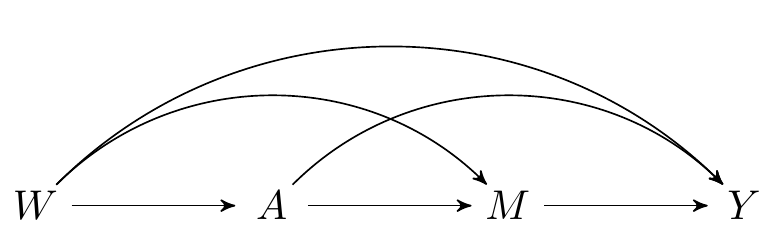
\includegraphics[width=0.8\linewidth]{01-preface_files/figure-latex/unnamed-chunk-4-1} 

}

\caption{Directed acyclic graph under *no intermediate confounders* of the mediator-outcome relation affected by treatment}\label{fig:unnamed-chunk-4}
\end{figure}

\hypertarget{intermediate-confounders}{%
\subsection{Intermediate confounders}\label{intermediate-confounders}}

\begin{figure}

{\centering \includegraphics[width=0.8\linewidth]{01-preface_files/figure-latex/unnamed-chunk-5-1} 

}

\caption{Directed acyclic graph under intermediate confounders of the mediator-outcome relation affected by treatment}\label{fig:unnamed-chunk-5}
\end{figure}

The above graphs can be interpreted as a \emph{non-parametric structural equation model}
(NPSEM), also known as \emph{structural causal model} (SCM):

\begin{align}
  W & = f_W(U_W)\\
  A & = f_A(W, U_A)\\
  Z & = f_Z(W, A, U_Z)\\
  M & = f_M(W, A, Z, U_M)\\
  Y & = f_Y(W, A, Z, M, U_Y)
\end{align}

\begin{itemize}
\tightlist
\item
  Here \(U=(U_W, U_A, U_Z, U_M, U_Y)\) is a vector of all unmeasured exogenous
  factors affecting the system
\item
  The functions \(f\) are assumed fixed but unknown
\item
  We posit this model as a system of equations that nature uses to generate the
  data
\item
  Therefore we leave the functions \(f\) unspecified (i.e., we do not know the
  true nature mechanisms)
\item
  Sometimes we know something: e.g., if \(A\) is randomized we know \(A=f_A(U_A)\)
  where \(U_A\) is the flip of a coin (i.e., independent of everything).
\end{itemize}

\hypertarget{counterfactuals}{%
\section{Counterfactuals}\label{counterfactuals}}

\begin{itemize}
\tightlist
\item
  Recall that we are interested in assessing how the pathways would behave under circumstances different from the observed circumstances
\item
  We operationalize this idea using \emph{counterfactual} variables
\item
  Counterfactuals are hypothetical random variables that would have been
  observed in an alternative world where something had happened, possibly
  contrary to fact 
\end{itemize}

\hypertarget{we-will-constantly-use-the-following-counterfactual-variables}{%
\subsection*{We will constantly use the following counterfactual variables:}\label{we-will-constantly-use-the-following-counterfactual-variables}}


\begin{itemize}
\tightlist
\item
  \(Y_a\) is a counterfactual variable in a hypothetical world where \(\P(A=a)=1\)
  with probability one for some valure \(a\)
\item
  \(Y_{a,m}\) is the counterfactual outcome in a world where \(\P(A=a,M=m)=1\)
\item
  \(M_a\) is the counterfactual variable representing the mediator in a world
  where \(\P(A=a)=1\).
\end{itemize}

\hypertarget{how-are-counterfactuals-defined}{%
\subsection{How are counterfactuals defined?}\label{how-are-counterfactuals-defined}}

\begin{itemize}
\tightlist
\item
  In the NPSEM framework, counterfactuals are quantities \emph{derived} from the
  model.
\item
  Once you define a change to the causal system, that change needs to be
  progragated downstream.

  \begin{itemize}
  \tightlist
  \item
    Example: modifying the system to make everyone receive XR-NTX yields
    counterfactual adherence, mediators, and outcomes.
  \end{itemize}
\item
  Take as example the DAG in Figure 1.2:
  \begin{align}
    A    &= a\\
    Z_a  &= f_Z(W, a, U_M)\\
    M_a  &= f_M(W, a, Z_a, U_M)\\
    Y_a  &= f_Y(W, a, Z_a, M_a, U_Y)\\
  \end{align}
\item
  We will also be interested in \_joint changes to the system:
  \begin{align}
    A    &= a\\
    Z_a  &= f_Z(W, a, U_M)\\
    M  &= m\\   
    Y_{a,m}  &= f_Y(W, a, Z_a, m, U_Y)\\
  \end{align}
\item
  And, perhaps more importantly, we will use \emph{nested counterfactuals}
\item
  For example, if \(A\) is binary, you can think of the following counterfactual
  \begin{align}
    A    &= 1\\
    Z_1  &= f_Z(W, 1, U_M)\\
    M  &= M_0\\ 
    Y_{1, M_0} &= f_Y(W, 1, Z_1, M_0, U_Y)\\
  \end{align}
\item
  \(Y_{1, M_0}\) is interpreted as \emph{the outcome for an individual in a
  hypothetical world where treatment was given but the mediator was held at the
  value it would have taken under no treatment}
\item
  Causal mediation effects are often defined in terms of the distribution of these
  nested counterfactuals.
\item
  That is, causal effects give you information about what would have happened
  \emph{in some hypothetical world} where the mediator and treatment mechanisms changed.
\end{itemize}

\hypertarget{estimands}{%
\chapter{Types of path-specific causal mediation effects}\label{estimands}}

\begin{itemize}
\tightlist
\item
  Controlled direct effects
\item
  Natural direct and indirect effects
\item
  Interventional direct and indirect effects
\end{itemize}

\begin{figure}

{\centering \includegraphics[width=0.8\linewidth]{02-effects-def_files/figure-latex/unnamed-chunk-1-1} 

}

\caption{Directed acyclic graph under *no intermediate confounders* of the mediator-outcome relation affected by treatment}\label{fig:unnamed-chunk-1}
\end{figure}

\hypertarget{controlled-direct-effects}{%
\section{Controlled direct effects}\label{controlled-direct-effects}}

\[\psi_{\text{CDE}} = \E(Y_{1,m} - Y_{0,m}) \]

\begin{figure}

{\centering 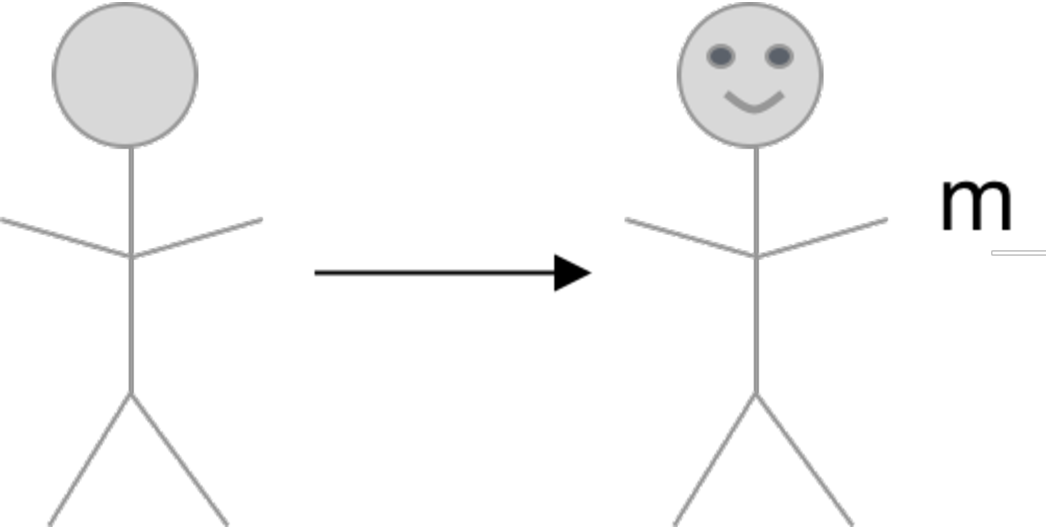
\includegraphics[width=0.5\linewidth]{/home/runner/work/ser2021_mediation_workshop/ser2021_mediation_workshop/img/graphic4a3} 

}

\end{figure}

\begin{itemize}
\tightlist
\item
  Set the mediator to a reference value \(M=m\) uniformly for everyone in the
  population
\item
  Compare \(A=1\) vs \(A=0\) with \(M=m\) fixed
\end{itemize}

\hypertarget{identification-assumptions}{%
\subsection{Identification assumptions:}\label{identification-assumptions}}

\begin{itemize}
\tightlist
\item
  Confounder assumptions:

  \begin{itemize}
  \tightlist
  \item
    \(A \indep Y_{a,m} \mid W\)
  \item
    \(M \indep Y_{a,m} \mid W, A\)
  \end{itemize}
\item
  Positivity assumptions:

  \begin{itemize}
  \tightlist
  \item
    \(\P(M = m \mid A=a, W) > 0 \text{  } a.e.\)
  \item
    \(\P(A=a \mid W) > 0 \text{  } a.e.\)
  \end{itemize}
\end{itemize}

Under the above identification assumptions, the controlled direct effect can be
identified:
\[ \E(Y_{1,m} - Y_{0,m}) = \E\{\color{ForestGreen}{\E(Y \mid A=1, M=m, W) - \E(Y \mid A=0, M=m, W)}\}\]

\begin{itemize}
\tightlist
\item
  For intuition about this formula in R, let's continue with a toy example:
\end{itemize}

\begin{lstlisting}[language=R]
n <- 1e6
w <- rnorm(n)
a <- rbinom(n, 1, 0.5)
m <- rnorm(n, w + a)
y <- rnorm(n, w + a + m)
\end{lstlisting}

\begin{itemize}
\tightlist
\item
  First we fit a correct model for the outcome
\end{itemize}

\begin{lstlisting}[language=R]
lm_y <- lm(y ~ m + a + w)
\end{lstlisting}

\begin{itemize}
\tightlist
\item
  Assume we would like the CDE at \(m=0\)
\item
  Then we generate predictions \[\color{ForestGreen}{\E(Y \mid A=1, M=m, W)}
  \text{ and }\color{ForestGreen}{\E(Y \mid A=0, M=m, W)}:\]
\end{itemize}

\begin{lstlisting}[language=R]
pred_y1 <- predict(lm_y, newdata = data.frame(a = 1, m = 0, w = w))
pred_y0 <- predict(lm_y, newdata = data.frame(a = 0, m = 0, w = w))
\end{lstlisting}

\begin{itemize}
\tightlist
\item
  Then we compute the difference between the predicted values
  \(\color{ForestGreen}{\E(Y \mid A=1, M=m, W) - \E(Y \mid A=0, M=m, W)}\), and
  average across values of \(W\)
\end{itemize}

\begin{lstlisting}[language=R]
## CDE at m = 0
mean(pred_y1 - pred_y0)
#> [1] 1.0009
\end{lstlisting}

\hypertarget{is-this-the-estimand-i-want}{%
\subsection{Is this the estimand I want?}\label{is-this-the-estimand-i-want}}

\begin{itemize}
\tightlist
\item
  Makes the most sense if can intervene directly on \(M\)

  \begin{itemize}
  \tightlist
  \item
    And can think of a policy that would set everyone to a single constant
    level \(m \in \mathcal{M}\).
  \item
    J. Pearl calls this \emph{prescriptive}.
  \item
    Can you think of an example?
  \item
    Air pollution, rescue inhaler dosage, hospital visits
  \item
    Does not provide a decomposition of the average treatment effect into
    direct and indirect effects
  \end{itemize}
\end{itemize}

\emph{What if our research question doesn't involve intervening directly on the
mediator?}

\emph{What if we want to decompose the average treatment effect into its direct and
indirect counterparts?}

\hypertarget{natural-direct-and-indirect-effects}{%
\section{Natural direct and indirect effects}\label{natural-direct-and-indirect-effects}}

Still using the same DAG as above,

\begin{itemize}
\tightlist
\item
  Recall the definition of the nested counterfactual
\end{itemize}

\begin{equation*}
    Y_{1, M_0} = f_Y(W, 1, M_0, U_Y)
\end{equation*}

\begin{itemize}
\item
  Interpreted as \emph{the outcome for an individual in a hypothetical world where
  treatment was given but the mediator was held at the value it would have
  taken under no treatment}

  \begin{figure}

  {\centering 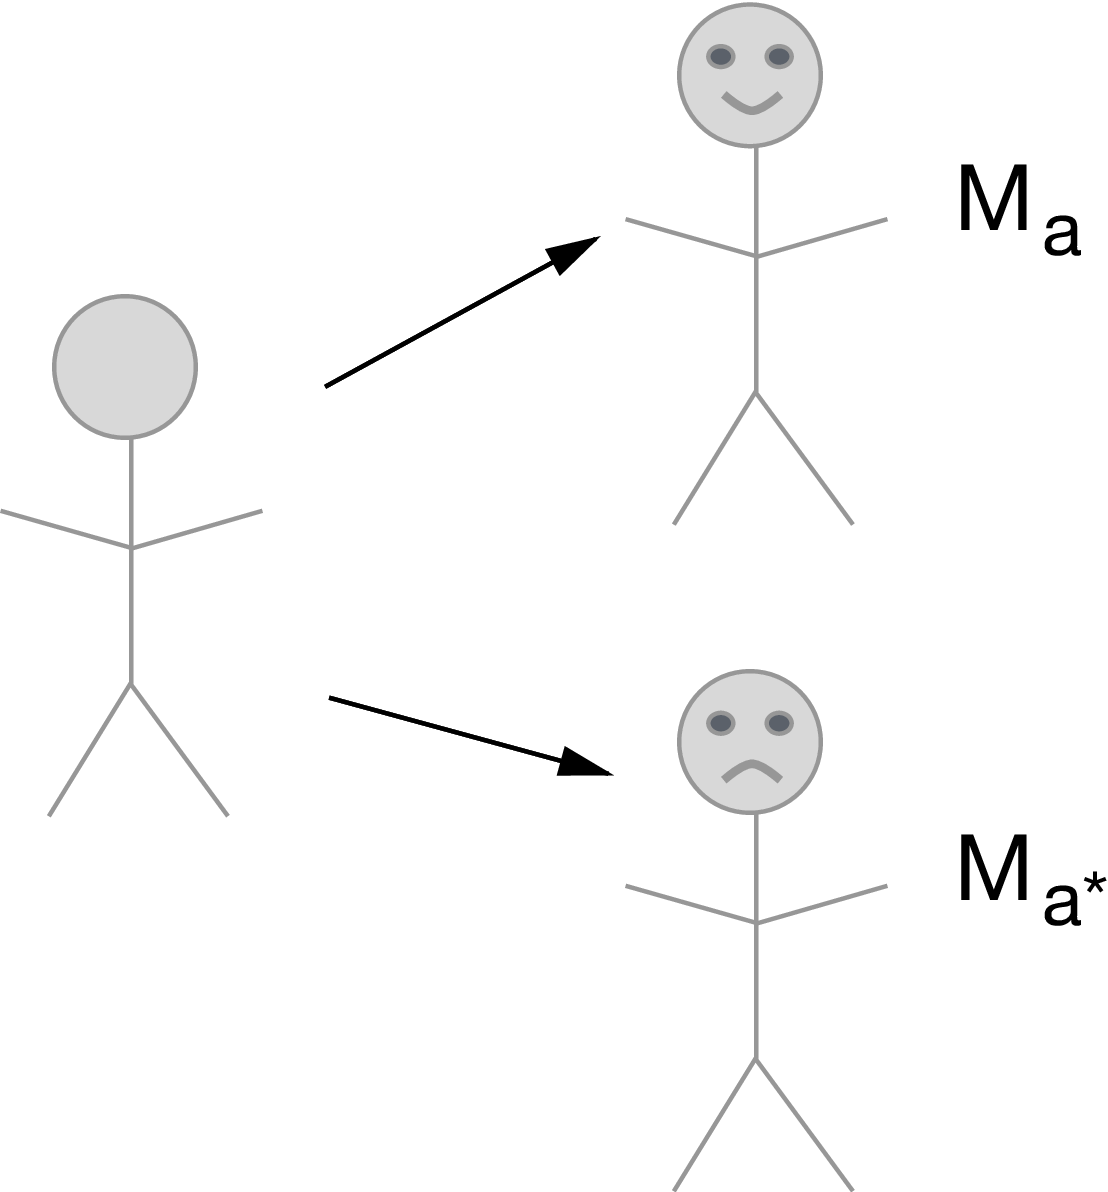
\includegraphics[width=0.5\linewidth]{/home/runner/work/ser2021_mediation_workshop/ser2021_mediation_workshop/img/graphic4a} 

  }

  \end{figure}
\item
  Recall that, because of the definition of counterfactuals
  \begin{equation*}
  Y_{1, M_1} = Y_1
  \end{equation*}
\end{itemize}

Then we can decompose the \emph{average treatment effect} \(E(Y_1-Y_0)\) as follows

\begin{equation*}
\E[Y_{1,M_1} - Y_{0,M_0}] = \underbrace{\E[Y_{\color{red}{1},\color{blue}{M_1}} -
    Y_{\color{red}{1},\color{blue}{M_0}}]}_{\text{natural indirect effect}} +
    \underbrace{\E[Y_{\color{blue}{1},\color{red}{M_0}} -
    Y_{\color{blue}{0},\color{red}{M_0}}]}_{\text{natural direct effect}}
\end{equation*}

\begin{itemize}
\tightlist
\item
  Natural direct effect (NDE): Varying treatment while keeping the mediator
  fixed at the value it would have taken under no treatment
\item
  Natural indirect effect (NIE): Varying the mediator from the value it would
  have taken under treatment to the value it would have taken under control,
  while keeping treatment fixed
\end{itemize}

\hypertarget{identification-assumptions-1}{%
\subsection{Identification assumptions:}\label{identification-assumptions-1}}

\begin{itemize}
\tightlist
\item
  \(A \indep Y_{a,m} \mid W\)
\item
  \(M \indep Y_{a,m} \mid W, A\)
\item
  \(A \indep M_a \mid W\)
\item
  \(M_0 \indep Y_{1,m} \mid W\)
\item
  and positivity assumptions
\end{itemize}

\hypertarget{cross-world-independence-assumption}{%
\subsection{Cross-world independence assumption}\label{cross-world-independence-assumption}}

What does \(M_0 \indep Y_{1,m} \mid W\) mean?

\begin{itemize}
\tightlist
\item
  Conditional on \(W\), knowledge of the mediator value in the absence of
  treatment, \(M_0\),
  provides no information about the outcome under treatment, \(Y_{1,m}\).
\item
  Can you think of a data-generating mechanism that would violate this
  assumption?
\item
  Example: in a randomized study, whenever we believe that treatment assignment
  works through adherence (i.e., almost
  always), we are violating this assumption (more on this later).
\item
  Cross-world assumptions are problematic for other reasons, including:

  \begin{itemize}
  \tightlist
  \item
    You can never design a randomized study where the assumption holds by
    design.
  \end{itemize}
\end{itemize}

\textbf{If the cross-world assumption holds, can write the NDE as a weighted average
of controlled direct effects at each level of \(M=m\).}

\[\E \sum_m \{\E(Y_{1,m} \mid W) - \E(Y_{0,m} \mid W)\} \P(M_{0}=m
\mid W)\]

\begin{itemize}
\tightlist
\item
  If CDE(\(m\)) is constant across \(m\), then CDE = NDE.
\end{itemize}

\hypertarget{identification-formula}{%
\subsection{Identification formula:}\label{identification-formula}}

\begin{itemize}
\item
  Under the above identification assumptions, the natural direct effect can be
  identified:
  \begin{equation*}
  \E(Y_{1,M_0} - Y_{0,M_0}) =
  \E[\color{Goldenrod}{\E\{}\color{ForestGreen}{\E(Y \mid A=1, M, W) -
  \E(Y \mid A=0, M, W)}\color{Goldenrod}{\mid A=0,W\}}]
  \end{equation*}
\item
  The natural indirect effect can be identified similarly.
\item
  Let's dissect this formula in \passthrough{\lstinline!R!}:
\end{itemize}

\begin{lstlisting}[language=R]
n <- 1e6
w <- rnorm(n)
a <- rbinom(n, 1, 0.5)
m <- rnorm(n, w + a)
y <- rnorm(n, w + a + m)
\end{lstlisting}

\begin{itemize}
\tightlist
\item
  First we fit a correct model for the outcome
\end{itemize}

\begin{lstlisting}[language=R]
lm_y <- lm(y ~ m + a + w)
\end{lstlisting}

\begin{itemize}
\tightlist
\item
  Then we generate predictions \[\color{ForestGreen}{\E(Y \mid A=1, M, W)}
  \text{ and }\color{ForestGreen}{\E(Y \mid A=0, M, W)}\] with \(A\) fixed but
  letting \(M\) and \(W\) take their observed
  values
\end{itemize}

\begin{lstlisting}[language=R]
pred_y1 <- predict(lm_y, newdata = data.frame(a = 1, m = m, w = w))
pred_y0 <- predict(lm_y, newdata = data.frame(a = 0, m = m, w = w))
\end{lstlisting}

\begin{itemize}
\tightlist
\item
  Then we compute the difference between the predicted values
  \[\color{ForestGreen}{\E(Y \mid A=1, M, W) - \E(Y \mid A=0, M, W)},\]
\item
  and use this difference as a pseudo-outcome in a regression on \(A\) and \(W\):
  \[\color{Goldenrod}{\E\{}\color{ForestGreen}{\E(Y \mid A=1, M, W) - \E(Y \mid
  A=0, M, W)}\color{Goldenrod}{\mid A=0,W\}}\]
\end{itemize}

\begin{lstlisting}[language=R]
pseudo <- pred_y1 - pred_y0
lm_pseudo <- lm(pseudo ~ a + w)
\end{lstlisting}

\begin{itemize}
\tightlist
\item
  Now we predict the value of this pseudo-outcome under \(A=0\), and average the
  result
\end{itemize}

\begin{lstlisting}[language=R]
pred_pseudo <- predict(lm_pseudo, newdata = data.frame(a = 0, w = w))
## NDE:
mean(pred_pseudo)
#> [1] 0.99655
\end{lstlisting}

\hypertarget{is-this-the-estimand-i-want-1}{%
\subsection{Is this the estimand I want?}\label{is-this-the-estimand-i-want-1}}

\begin{itemize}
\tightlist
\item
  Makes sense to intervene on \(A\) but not directly on \(M\).
\item
  Want to understand a natural mechanism underlying an association/ total
  effect. J. Pearl calls this \emph{descriptive}.
\item
  NDE + NIE = total effect (ATE).
\item
  Okay with the assumptions.
\end{itemize}

\emph{What if our data structure involves a post-treatment confounder of the
mediator-outcome relationship (e.g., adherence)?}

\begin{figure}

{\centering \includegraphics[width=0.8\linewidth]{02-effects-def_files/figure-latex/unnamed-chunk-12-1} 

}

\caption{Directed acyclic graph under intermediate confounders of the mediator-outcome relation affected by treatment}\label{fig:unnamed-chunk-12}
\end{figure}

\begin{figure}

{\centering 
\includegraphics[width=1\linewidth]{/home/runner/work/ser2021_mediation_workshop/ser2021_mediation_workshop/img/ctndag} 

}

\end{figure}

\hypertarget{unidentifiability-of-the-nde-and-nie-in-this-setting}{%
\subsection{Unidentifiability of the NDE and NIE in this setting}\label{unidentifiability-of-the-nde-and-nie-in-this-setting}}

\begin{itemize}
\tightlist
\item
  In this example, natural direct and indirect effects are unidentifiable from observed data \(O=(W,A,Z,M,Y)\).
\item
  The reason for this is that the cross-world counterfactual
  assumption
  \begin{equation*}
  Y_{1,m}\indep M_0\mid W
  \end{equation*}
  does not hold in the above directed acyclic graph.
\item
  Technically, the reason for this is that an intervention setting \(A=1\)
  (necessary for the definition of \(Y_{1,m}\)) induces a counterfactual variable
  \(Z_1\).
\item
  Likewise, an intervention setting \(A=0\) (necessary for the definition of
  \(M_0\)) induces a counterfactual \(Z_0\).
\item
  The variables \(Z_1\) and \(Z_0\) are correlated because they share unmeasured
  common causes, \(U_Z\).
\item
  The variable \(Z_1\) is correlated with \(Y_{1,m}\), and the variable \(Z_0\) is
  correlated with \(M_0\), because they are counterfactual outcomes in the same
  hypothetical worlds.
\item
  To see this in the definition of counterfactual from a causal structural
  model:
  \begin{align*}
  Y_{1,m} &= f_Y(W, 1, Z_1, m, U_Y), \text{ and }\\
  M_0 &= f_M(W, 0, Z_0, U_M)\\
  \end{align*}
  are correlated even after adjusting for \(W\) by virtue of \(Z_1\) and \(Z_0\) being
  correlated.
\end{itemize}

Note: CDEs are still identified in this setting. They can be identified and
estimated similarly to a longitudinal data sructure with a two-time-point
intervention.

\hypertarget{interventional-indirect-effects}{%
\section{Interventional (in)direct effects}\label{interventional-indirect-effects}}

\begin{itemize}
\tightlist
\item
  Let \(G_a\) denote a random draw from the distribution of \(M_a \mid W\)
\item
  Define the counterfactual \(Y_{1,G_0}\) as the counterfactual
  variable in a hypothetical world where \(A\) is set \(A=1\) and \(M\) is
  set to \(M=G_0\) with probability one.
\end{itemize}

\begin{figure}

{\centering 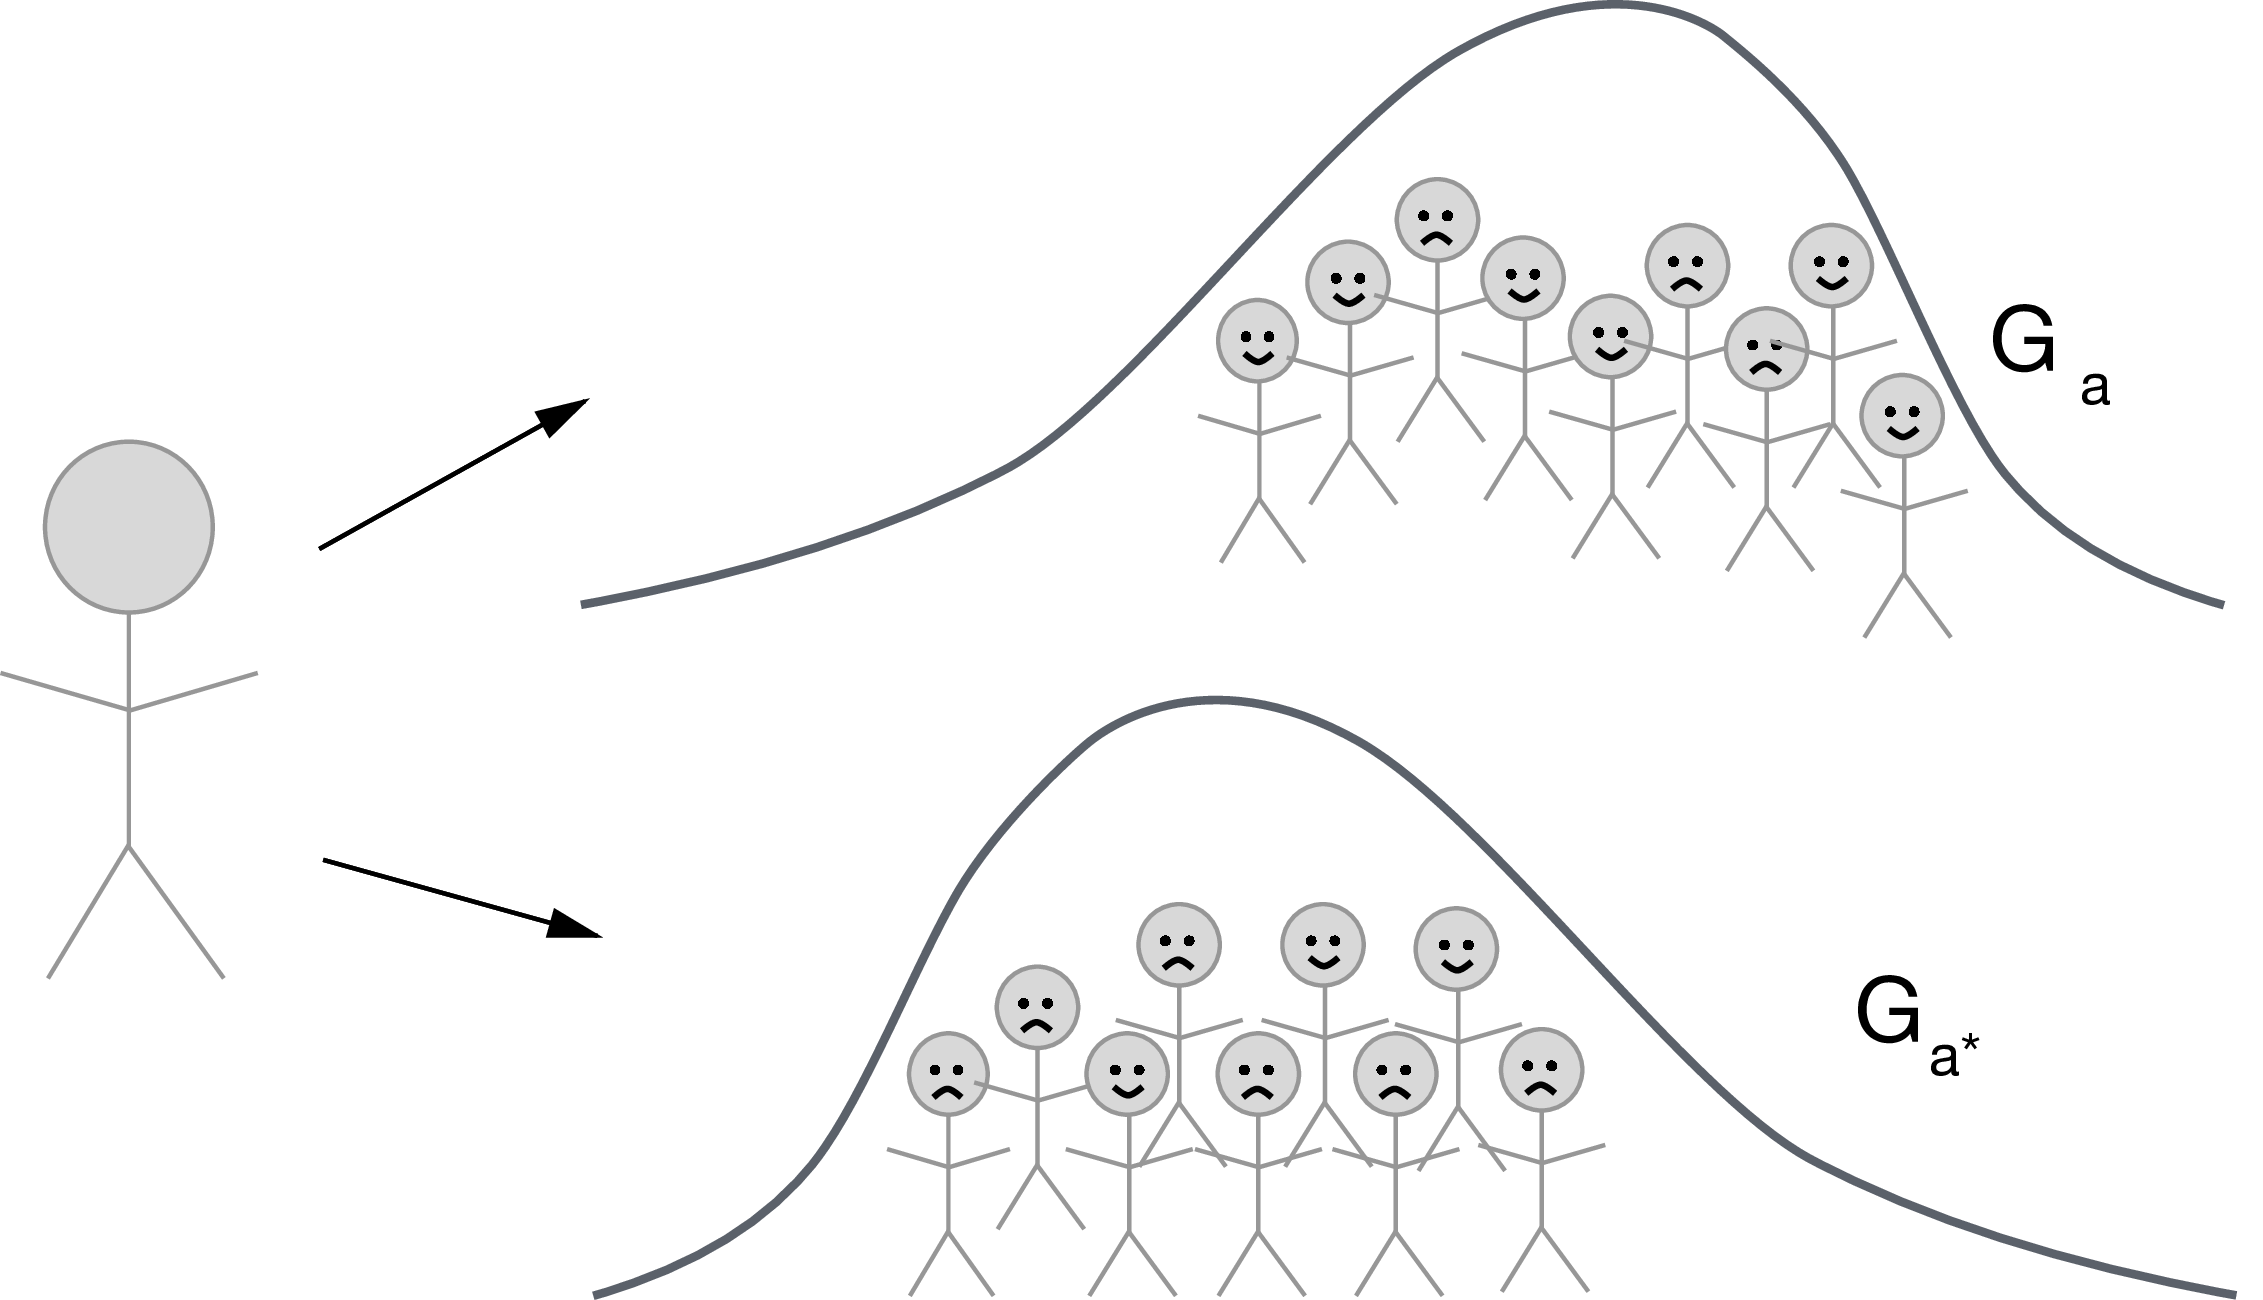
\includegraphics[width=0.5\linewidth]{/home/runner/work/ser2021_mediation_workshop/ser2021_mediation_workshop/img/graphic4b} 

}

\end{figure}

\begin{itemize}
\tightlist
\item
  Define \(Y_{0,G_0}\) and \(Y_{1,G_1}\) similarly
\item
  Then we can define:
  \begin{equation*}
  \E[Y_{1,G_1} - Y_{0,G_0}] = \underbrace{\E[Y_{\color{red}{1},\color{blue}{G_1}} -
    Y_{\color{red}{1},\color{blue}{G_0}}]}_{\text{interventional indirect effect}} +
    \underbrace{\E[Y_{\color{blue}{1},\color{red}{G_0}} -
    Y_{\color{blue}{0},\color{red}{G_0}}]}_{\text{interventional direct effect}}
  \end{equation*}
\item
  Note that \(\E[Y_{1,G_1} - Y_{0,G_0}]\) is still a \emph{total effect} of treatment,
  even if it is different from the ATE \(\E[Y_{1} - Y_{0}]\)
\item
  We gain in the ability to solve a problem, but lose in terms of interpretation
  of the causal effect (cannot decompose the ATE)
\end{itemize}

\hypertarget{an-alternative-definition-of-the-effects}{%
\subsection{An alternative definition of the effects:}\label{an-alternative-definition-of-the-effects}}

\begin{itemize}
\tightlist
\item
  Above we defined \(G_a\) as a random draw from the distribution of \(M_a \mid W\)
\item
  What if instead we define \(G_a\) as a random draw from the distribution of \(M_a \mid (Z_a,W)\)
\item
  It turns out the indirect effect defined in this way only measures the path
  \(A\rightarrow M \rightarrow Y\), and not the path \(A\rightarrow Z\rightarrow M \rightarrow Y\)
\item
  There may be important reasons to choose one over another (e.g., survival
  analyses where we want the distribution conditional on \(Z\), instrumental
  variable designs where it doesn't make sense to condition on \(Z\))
\end{itemize}

\hypertarget{identification-assumptions-2}{%
\subsection{Identification assumptions:}\label{identification-assumptions-2}}

\begin{itemize}
\tightlist
\item
  \(A \indep Y_{a,m} \mid W\)
\item
  \(M \indep Y_{a,m} \mid W, A, Z\)
\item
  \(A \indep M_a \mid W\)
\item
  and positivity assumptions.
\end{itemize}

Under these assumptions, the population interventional direct and indirect effect is identified:
\begin{align*}
  \E&(Y_{a, G_{a'}}) = \\
    &\E\left[\color{Purple}{\E\left\{\color{Goldenrod}{\sum_z}
    \color{ForestGreen}{\E(Y \mid A=a, Z=z, M, W)}
    \color{Goldenrod}{\P(Z=z \mid A=a, W)}\mid A=a', W\right\}}\right]
\end{align*}

\begin{itemize}
\tightlist
\item
  Let's dissect this formula in \passthrough{\lstinline!R!}:
\end{itemize}

\begin{lstlisting}[language=R]
n <- 1e6
w <- rnorm(n)
a <- rbinom(n, 1, 0.5)
z <- rbinom(n, 1, 0.5 + 0.2 * a)
m <- rnorm(n, w + a - z)
y <- rnorm(n, w + a + z + m)
\end{lstlisting}

\begin{itemize}
\tightlist
\item
  Let us compute \(\E(Y_{1, G_0})\) (so that \(a = 1\), and \(a'=0\)).
\item
  First, fit a regression model for the outcome, and compute
  \[\color{ForestGreen}{\E(Y \mid A=a, Z=z, M, W)}\] for all values of \(z\)
\end{itemize}

\begin{lstlisting}[language=R]
lm_y <- lm(y ~ m + a + z + w)
pred_a1z0 <- predict(lm_y, newdata = data.frame(m = m, a = 1, z = 0, w = w))
pred_a1z1 <- predict(lm_y, newdata = data.frame(m = m, a = 1, z = 1, w = w))
\end{lstlisting}

\begin{itemize}
\tightlist
\item
  Now we fit the true model for \(Z \mid A, W\) and get the conditional
  probability that \(Z=1\) fixing \(A=1\)
\end{itemize}

\begin{lstlisting}[language=R]
prob_z <- lm(z ~ a)
pred_z <- predict(prob_z, newdata = data.frame(a = 1))
\end{lstlisting}

\begin{itemize}
\tightlist
\item
  Now we compute the following pseudo-outcome:
  \[\color{Goldenrod}{\sum_z}\color{ForestGreen}{\E(Y \mid A=a, Z=z, M, W)}
  \color{Goldenrod}{\P(Z=z \mid A=a, w)}\]
\end{itemize}

\begin{lstlisting}[language=R]
pseudo_out <- pred_a1z0 * (1 - pred_z) + pred_a1z1 * pred_z
\end{lstlisting}

\begin{itemize}
\tightlist
\item
  Now we regress this pseudo-outcome on \(A,W\), and compute the predictions
  setting \(A=0\), that is, \[\color{Purple}{\E\left\{\color{Goldenrod}{\sum_z}
  \color{ForestGreen}{\E(Y \mid A=a, Z=z, M, W)}
  \color{Goldenrod}{\P(Z=z \mid A=a, w)}\mid A=a', W\right\}}\]
\end{itemize}

\begin{lstlisting}[language=R]
fit_pseudo <- lm(pseudo_out ~ a + w)
pred_pseudo <- predict(fit_pseudo, data.frame(a = 0, w = w))
\end{lstlisting}

\begin{itemize}
\tightlist
\item
  And finally, just average those predictions!
\end{itemize}

\begin{lstlisting}[language=R]
## Mean(Y(1, G(0)))
mean(pred_pseudo)
#> [1] 1.1979
\end{lstlisting}

\begin{itemize}
\tightlist
\item
  This was for \((a,a')=(1,0)\). Can do the same with \((a,a')=(1,1)\), and
  \((a,a')=(0,0)\) to obtain an effect decomposition
\end{itemize}

\begin{equation*}
  \E[Y_{1,G_1} - Y_{0,G_0}] = \underbrace{\E[Y_{\color{red}{1},
    \color{blue}{G_1}} -
    Y_{\color{red}{1},
    \color{blue}{G_0}}]}_{\text{interventional indirect effect}} +
    \underbrace{\E[Y_{\color{blue}{1},\color{red}{G_0}} -
    Y_{\color{blue}{0},
    \color{red}{G_0}}]}_{\text{interventional direct effect}}
\end{equation*}

\hypertarget{is-this-the-estimand-i-want-2}{%
\subsection{Is this the estimand I want?}\label{is-this-the-estimand-i-want-2}}

\begin{itemize}
\tightlist
\item
  Makes sense to intervene on \(A\) but not directly on \(M\).
\item
  Goal is to understand a natural mechanism underlying an association or total
  effect.
\item
  Okay with the assumptions!
\end{itemize}

\hypertarget{estimand-summary}{%
\section{Estimand Summary}\label{estimand-summary}}

\begin{figure}

{\centering 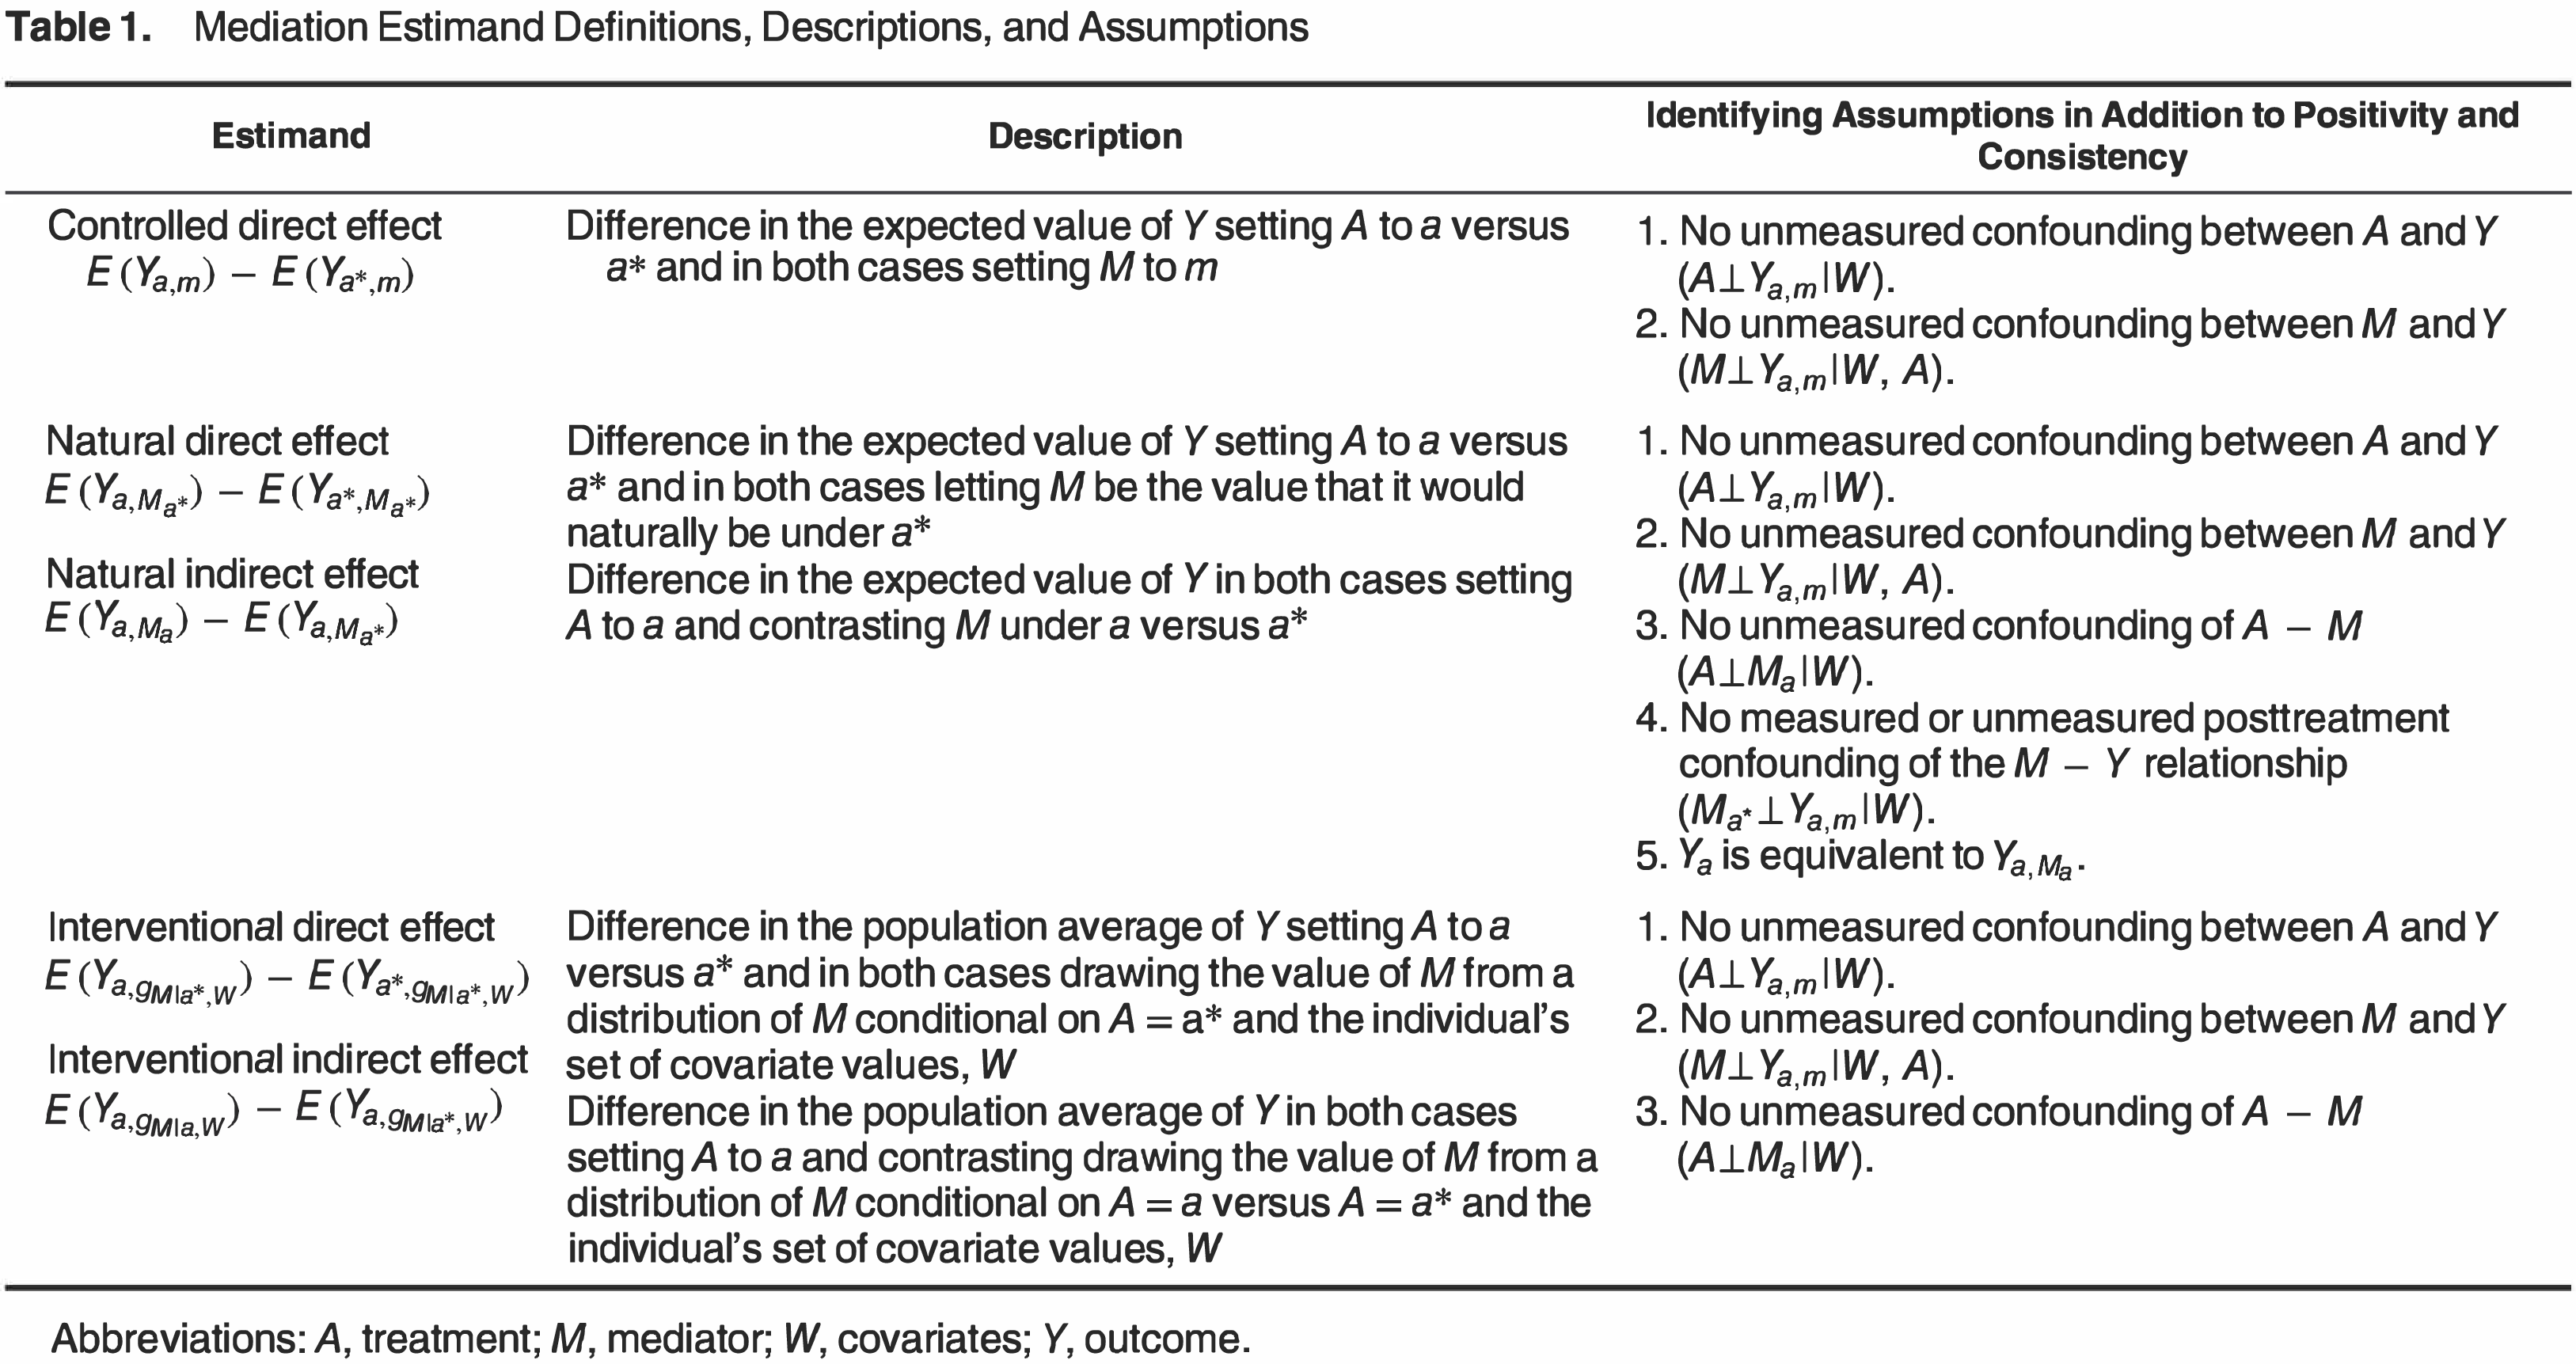
\includegraphics[width=1.25\linewidth]{/home/runner/work/ser2021_mediation_workshop/ser2021_mediation_workshop/img/table1} 

}

\caption{Excerpted from @rudolph2019causal}\label{fig:unnamed-chunk-21}
\end{figure}

\hypertarget{stochastic}{%
\chapter{Stochastic direct and indirect effects}\label{stochastic}}

\hypertarget{definition-of-the-effects}{%
\section{Definition of the effects}\label{definition-of-the-effects}}

Consider the following directed acyclic graph.

\begin{figure}

{\centering \includegraphics[width=0.8\linewidth]{03-stochastic_files/figure-latex/unnamed-chunk-1-1} 

}

\caption{Directed acyclic graph under no intermediate confounders of the mediator-outcome relation affected by treatment}\label{fig:unnamed-chunk-1}
\end{figure}

\hypertarget{motivation-for-stochastic-interventions}{%
\section{Motivation for stochastic interventions}\label{motivation-for-stochastic-interventions}}

\begin{itemize}
\tightlist
\item
  So far we have discussed controlled, natural, and interventional (in)direct effects
\item
  These effects require that \(0 < \P(A=1\mid W) < 1\)
\item
  They are defined only for binary exposures
\item
  \emph{What can we do when the positivity assumption does not hold or the exposure
  is continuous?}
\item
  Solution: we can use stochastic effects
\end{itemize}

\hypertarget{definition-of-stochastic-effects}{%
\section{Definition of stochastic effects}\label{definition-of-stochastic-effects}}

There are two possible ways of defining stochastic effects:

\begin{itemize}
\tightlist
\item
  Consider the effect of an intervention where the exposure is drawn from a
  distribution

  \begin{itemize}
  \tightlist
  \item
    For example incremental propensity score interventions
  \end{itemize}
\end{itemize}

\begin{itemize}
\tightlist
\item
  Consider the effect of an intervention where the post-intervention exposure is
  a function of the actually received exposure

  \begin{itemize}
  \tightlist
  \item
    For example modified treatment policies
  \end{itemize}
\item
  In both cases \(A \mid W\) is a non-deterministic intervention, thus the name
  \emph{stochastic intervention}
\end{itemize}

\hypertarget{ipsi}{%
\subsection{\texorpdfstring{Example: incremental propensity score interventions (IPSI) \citep{kennedy2018nonparametric}}{Example: incremental propensity score interventions (IPSI) {[}@kennedy2018nonparametric{]}}}\label{ipsi}}

\hypertarget{definition-of-the-intervention}{%
\subsubsection*{Definition of the intervention}\label{definition-of-the-intervention}}


\begin{itemize}
\tightlist
\item
  Assume \(A\) is binary, and \(\P(A=1\mid W=w) = g(1\mid w)\) is the propensity score
\item
  Consider an intervention in which each individual receives the intervention
  with probability \(g_\delta(1\mid w)\), equal to
  \begin{equation*}
    g_\delta(1\mid w)=\frac{\delta g(1\mid w)}{\delta g(1\mid w) +
    1 - g(1\mid w)}
  \end{equation*}
\item
  e.g., draw the post-intervention exposure from a Bernoulli variable with
  probability \(g_\delta(1\mid w)\)
\item
  The value \(\delta\) is user given
\item
  Let \(A_\delta\) denote the post-intervention exposure distribution
\item
  Some algebra shows that \(\delta\) is an odds ratio comparing the pre- and
  post-intervention exposure distributions
  \begin{equation*}
    \delta = \frac{\text{odds}(A_\delta = 1\mid W=w)}
    {\text{odds}(A = 1\mid W=w)}
  \end{equation*}
\item
  Interpretation: \emph{what would happen in a
  world where the odds of receiving treatment is increased by \(\delta\)}
\item
  Let \(Y_{A_\delta}\) denote the outcome in this hypothetical world
\end{itemize}

\hypertarget{illustrative-application-for-ipsis}{%
\subsubsection{Illustrative application for IPSIs}\label{illustrative-application-for-ipsis}}

\begin{itemize}
\tightlist
\item
  Consider the effect of participation in sports on children's BMI
\item
  Mediation through snacking, exercising, etc.
\item
  Intervention: for each individual, increase the odds of participating in
  sports by \(\delta=2\)
\item
  The post-intervention exposure is a draw \(A_\delta\) from a Bernoulli
  distribution with probability \(g_\delta(1\mid w)\)
\end{itemize}

\hypertarget{example-modified-treatment-policies-mtp-diaz2020causal}{%
\subsection*{\texorpdfstring{Example: modified treatment policies (MTP) \citep{diaz2020causal}}{Example: modified treatment policies (MTP) {[}@diaz2020causal{]}}}\label{example-modified-treatment-policies-mtp-diaz2020causal}}


\hypertarget{definition-of-the-intervention-1}{%
\subsubsection*{Definition of the intervention}\label{definition-of-the-intervention-1}}


\begin{itemize}
\tightlist
\item
  Consider a continuous exposure \(A\) taking values in the real numbers
\item
  Consider an intervention that assigns exposure as \(A_\delta = A - \delta\)
\item
  Example: \(A\) is pollution measured as \(PM_{2.5}\) and you are interested in an
  intervention that reduces \(PM_{2.5}\) concentration by some amount \(\delta\)
\end{itemize}

\hypertarget{mediation-analysis-for-stochastic-interventions}{%
\subsection{Mediation analysis for stochastic interventions}\label{mediation-analysis-for-stochastic-interventions}}

\begin{itemize}
\item
  The total effect of an IPSI can be computed as a contrast of the outcome under
  intervention vs no intervention:
  \begin{equation*}
    \psi = \E[Y_{A_\delta} - Y]
  \end{equation*}
\item
  Recall the NPSEM
  \begin{align}
    W & = f_W(U_W)\\
    A & = f_A(W, U_A)\\
    M & = f_M(W, A, U_M)\\
    Y & = f_Y(W, A, M, U_Y)
  \end{align}
\item
  From this we have
  \begin{align*}
  M_{A_\delta} & = f_M(W, A_\delta, U_M)\\
  Y_{A_\delta} & = f_Y(W, A_\delta, M_{A_\delta}, U_Y)
  \end{align*}
\item
  Thus, we have \(Y_{A_\delta} = Y_{A_\delta, M_{A_\delta}}\) and \(Y = Y_{A,M_{A}}\)
\item
  Let us introduce the counterfactual \(Y_{A_\delta, M}\), interpreted as the
  outcome observed in a world where the intervention on \(A\) is performed but the
  mediator is fixed at the value it would have taken under no intervention:
  \[Y_{A_\delta, M}  = f_Y(W, A_\delta, M_{A_\delta}, U_Y)\]
\item
  Then we can decompose the total effect into:
  \begin{align*}
    \E[Y&_{A_\delta,M_{A_\delta}} - Y_{A,M_A}] = \\
    &\underbrace{\E[Y_{\color{red}{A_\delta},\color{blue}{M_{A_\delta}}} -
      Y_{\color{red}{A_\delta},\color{blue}{M}}]}_{\text{stochastic natural indirect effect}} +
      \underbrace{\E[Y_{\color{blue}{A_\delta},\color{red}{M}} -
      Y_{\color{blue}{A},\color{red}{M}}]}_{\text{stochastic natural direct effect}}
  \end{align*}
\end{itemize}

\hypertarget{identification-assumptions-3}{%
\section{Identification assumptions}\label{identification-assumptions-3}}

\begin{itemize}
\tightlist
\item
  Confounder assumptions:

  \begin{itemize}
  \tightlist
  \item
    \(A \indep Y_{a,m} \mid W\)
  \item
    \(M \indep Y_{a,m} \mid W, A\)
  \end{itemize}
\item
  No confounder of \(M\rightarrow Y\) affected by \(A\)
\item
  Positivity assumptions:

  \begin{itemize}
  \tightlist
  \item
    If \(g_\delta(a \mid w)>0\) then \(g(a \mid w)>0\)
  \item
    If \(\P(Z=z\mid W=w)>0\) then \(\P(Z=z\mid A=a,W=w)>0\)
  \end{itemize}
\end{itemize}

Under these assumptions, stochastic effects are identified as follows

\begin{itemize}
\item
  The indirect effect can be identified as follows
  \begin{align*}
  \E&(Y_{A_\delta} - Y_{A_\delta, M}) =\\
  &\E\left[\color{Goldenrod}{\sum_{a}\color{ForestGreen}{\{\E(Y\mid A=a, W)-\E(Y\mid A=a, M, W)\}}g_\delta(a\mid W)}\right]
  \end{align*}
\item
  The direct effect can be identified as follows
  \begin{align*}
  \E&(Y_{A_\delta} - Y_{A_\delta, M}) =\\
  &\E\left[\color{Goldenrod}{\sum_{a}\color{ForestGreen}{\{\E(Y\mid A=a, M, W) - Y\}}g_\delta(a\mid W)}\right]
  \end{align*}
\item
  Let's dissect the formula for the indirect effect in R:
\end{itemize}

\begin{lstlisting}[language=R]
n <- 1e6
w <- rnorm(n)
a <- rbinom(n, 1, plogis(1 + w))
m <- rnorm(n, w + a)
y <- rnorm(n, w + a + m)
\end{lstlisting}

\begin{itemize}
\tightlist
\item
  First, fit regressions of the outcome on \((A,W)\) and \((M,A,W)\):
\end{itemize}

\begin{lstlisting}[language=R]
fit_y1 <- lm(y ~ m + a + w)
fit_y2 <- lm(y ~ a + w)
\end{lstlisting}

\begin{itemize}
\tightlist
\item
  Get predictions fixing \(A=a\) for all possible values \(a\)
\end{itemize}

\begin{lstlisting}[language=R]
pred_y1_a1 <- predict(fit_y1, newdata = data.frame(a = 1, m, w))
pred_y1_a0 <- predict(fit_y1, newdata = data.frame(a = 0, m, w))
pred_y2_a1 <- predict(fit_y2, newdata = data.frame(a = 1, w))
pred_y2_a0 <- predict(fit_y2, newdata = data.frame(a = 0, w))
\end{lstlisting}

\begin{itemize}
\tightlist
\item
  Compute
  \[\color{ForestGreen}{\{\E(Y\mid A=a, W)-\E(Y\mid A=a, M, W)\}}\]
  for each value \(a\)
\end{itemize}

\begin{lstlisting}[language=R]
pseudo_a1 <- pred_y2_a1 - pred_y1_a1
pseudo_a0 <- pred_y2_a0 - pred_y1_a0
\end{lstlisting}

\begin{itemize}
\tightlist
\item
  Estimate the propensity score \(g(1\mid w)\) and evaluate the post-intervention
  propensity score \(g_\delta(1\mid w)\)
\end{itemize}

\begin{lstlisting}[language=R]
pscore_fit <- glm(a ~ w, family = binomial())
pscore <- predict(pscore_fit, type = 'response')
## How do the intervention vs observed propensity score compare
pscore_delta <- 2 * pscore / (2 * pscore + 1 - pscore)
\end{lstlisting}

\begin{itemize}
\tightlist
\item
  What do the post-intervention propensity scores look like?
\end{itemize}

\begin{lstlisting}[language=R]
plot(pscore, pscore_delta, xlab = 'Observed prop. score',
     ylab = 'Prop. score under intervention')
abline(0, 1)
\end{lstlisting}

\begin{center}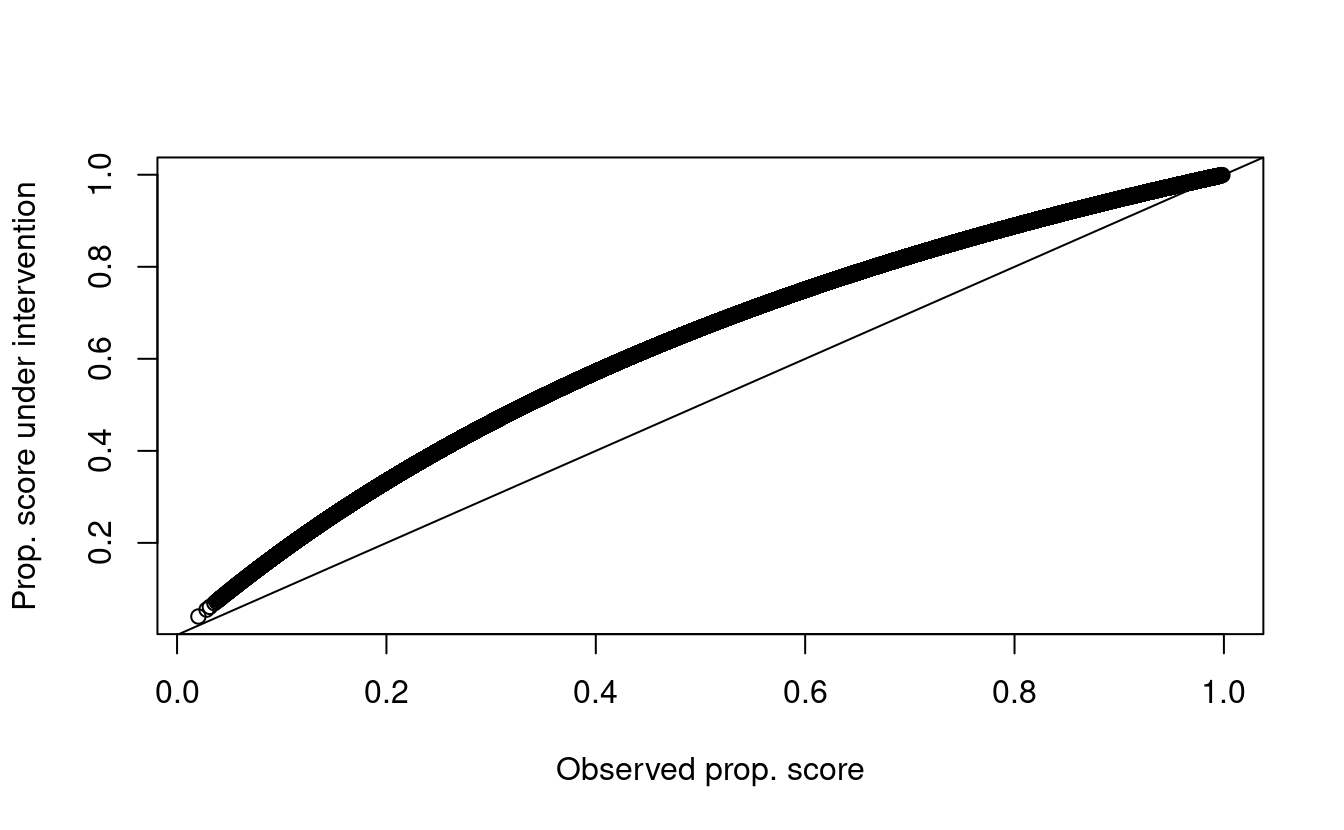
\includegraphics[width=0.8\linewidth]{03-stochastic_files/figure-latex/unnamed-chunk-7-1} \end{center}

\hypertarget{what-are-the-odds-of-exposure-under-intervention-vs-real-world}{%
\section{What are the odds of exposure under intervention vs real world?}\label{what-are-the-odds-of-exposure-under-intervention-vs-real-world}}

\begin{lstlisting}[language=R]
odds <- (pscore_delta / (1 - pscore_delta)) / (pscore / (1 - pscore))
summary(odds)
#>    Min. 1st Qu.  Median    Mean 3rd Qu.    Max. 
#>       2       2       2       2       2       2
\end{lstlisting}

\begin{itemize}
\tightlist
\item
  Compute the sum
  \[\color{Goldenrod}{\sum_{a}\color{ForestGreen}{\{\E(Y\mid A=a, W)-\E(Y\mid A=a, M, W)\}}g_\delta(a\mid W)}\]
\end{itemize}

\begin{lstlisting}[language=R]
indirect <- pseudo_a1 * pscore_delta + pseudo_a0 * (1 - pscore_delta)
\end{lstlisting}

\begin{itemize}
\tightlist
\item
  The average of this value is the indirect effect
\end{itemize}

\begin{lstlisting}[language=R]
## E[Y(Adelta) - Y(Adelta, M)]
mean(indirect)
#> [1] 0.1091
\end{lstlisting}

\begin{itemize}
\item
  The direct effect is
  \begin{align*}
  \E&(Y_{A_\delta} - Y_{A_\delta, M}) =\\
  &\E\left[\color{Goldenrod}{\sum_{a}\color{ForestGreen}{\{\E(Y\mid A=a, M, W) - Y\}}g_\delta(a\mid W)}\right]
  \end{align*}
\item
  Which can be computed as
\end{itemize}

\begin{lstlisting}[language=R]
direct <- (pred_y1_a1 - y) * pscore_delta +
       (pred_y1_a0 - y) * (1 - pscore_delta)
mean(direct)
#> [1] 0.10934
\end{lstlisting}

\hypertarget{summary}{%
\section{Summary}\label{summary}}

\begin{itemize}
\tightlist
\item
  Stochastic (in)direct effects

  \begin{itemize}
  \tightlist
  \item
    Relax the positivity assumption
  \item
    Can be defined for non-binary exposures
  \item
    Do not require a cross-world assumption
  \end{itemize}
\item
  Still require the absence of intermediate confounders

  \begin{itemize}
  \tightlist
  \item
    But, compared to the NDE and NIE, we can design a randomized study where
    identifiability assumptions hold, at least in principle
  \item
    There is a version of these effects that can accomodate intermediate
    confounders \citep{hejazi2020nonparametric}
  \item
    \passthrough{\lstinline!R!} implementation to be released soon\ldots stay tuned!
  \end{itemize}
\end{itemize}

\hypertarget{estimandirl}{%
\chapter{How to choose an estimand: Real-world example}\label{estimandirl}}

\hypertarget{comparative-effectivness-of-two-medications-for-opioid-use-disorder-oud}{%
\section{Comparative effectivness of two medications for opioid use disorder (OUD)}\label{comparative-effectivness-of-two-medications-for-opioid-use-disorder-oud}}

\begin{figure}

{\centering 
\includegraphics[width=1\linewidth]{/home/runner/work/ser2021_mediation_workshop/ser2021_mediation_workshop/img/ctndag} 

}

\end{figure}

\emph{Motivation}: Opposite overall treatment effects for homeless versus
nonhomeless participants. This application was explored in detail by
\citet{rudolph2020explaining}.

\begin{figure}

{\centering 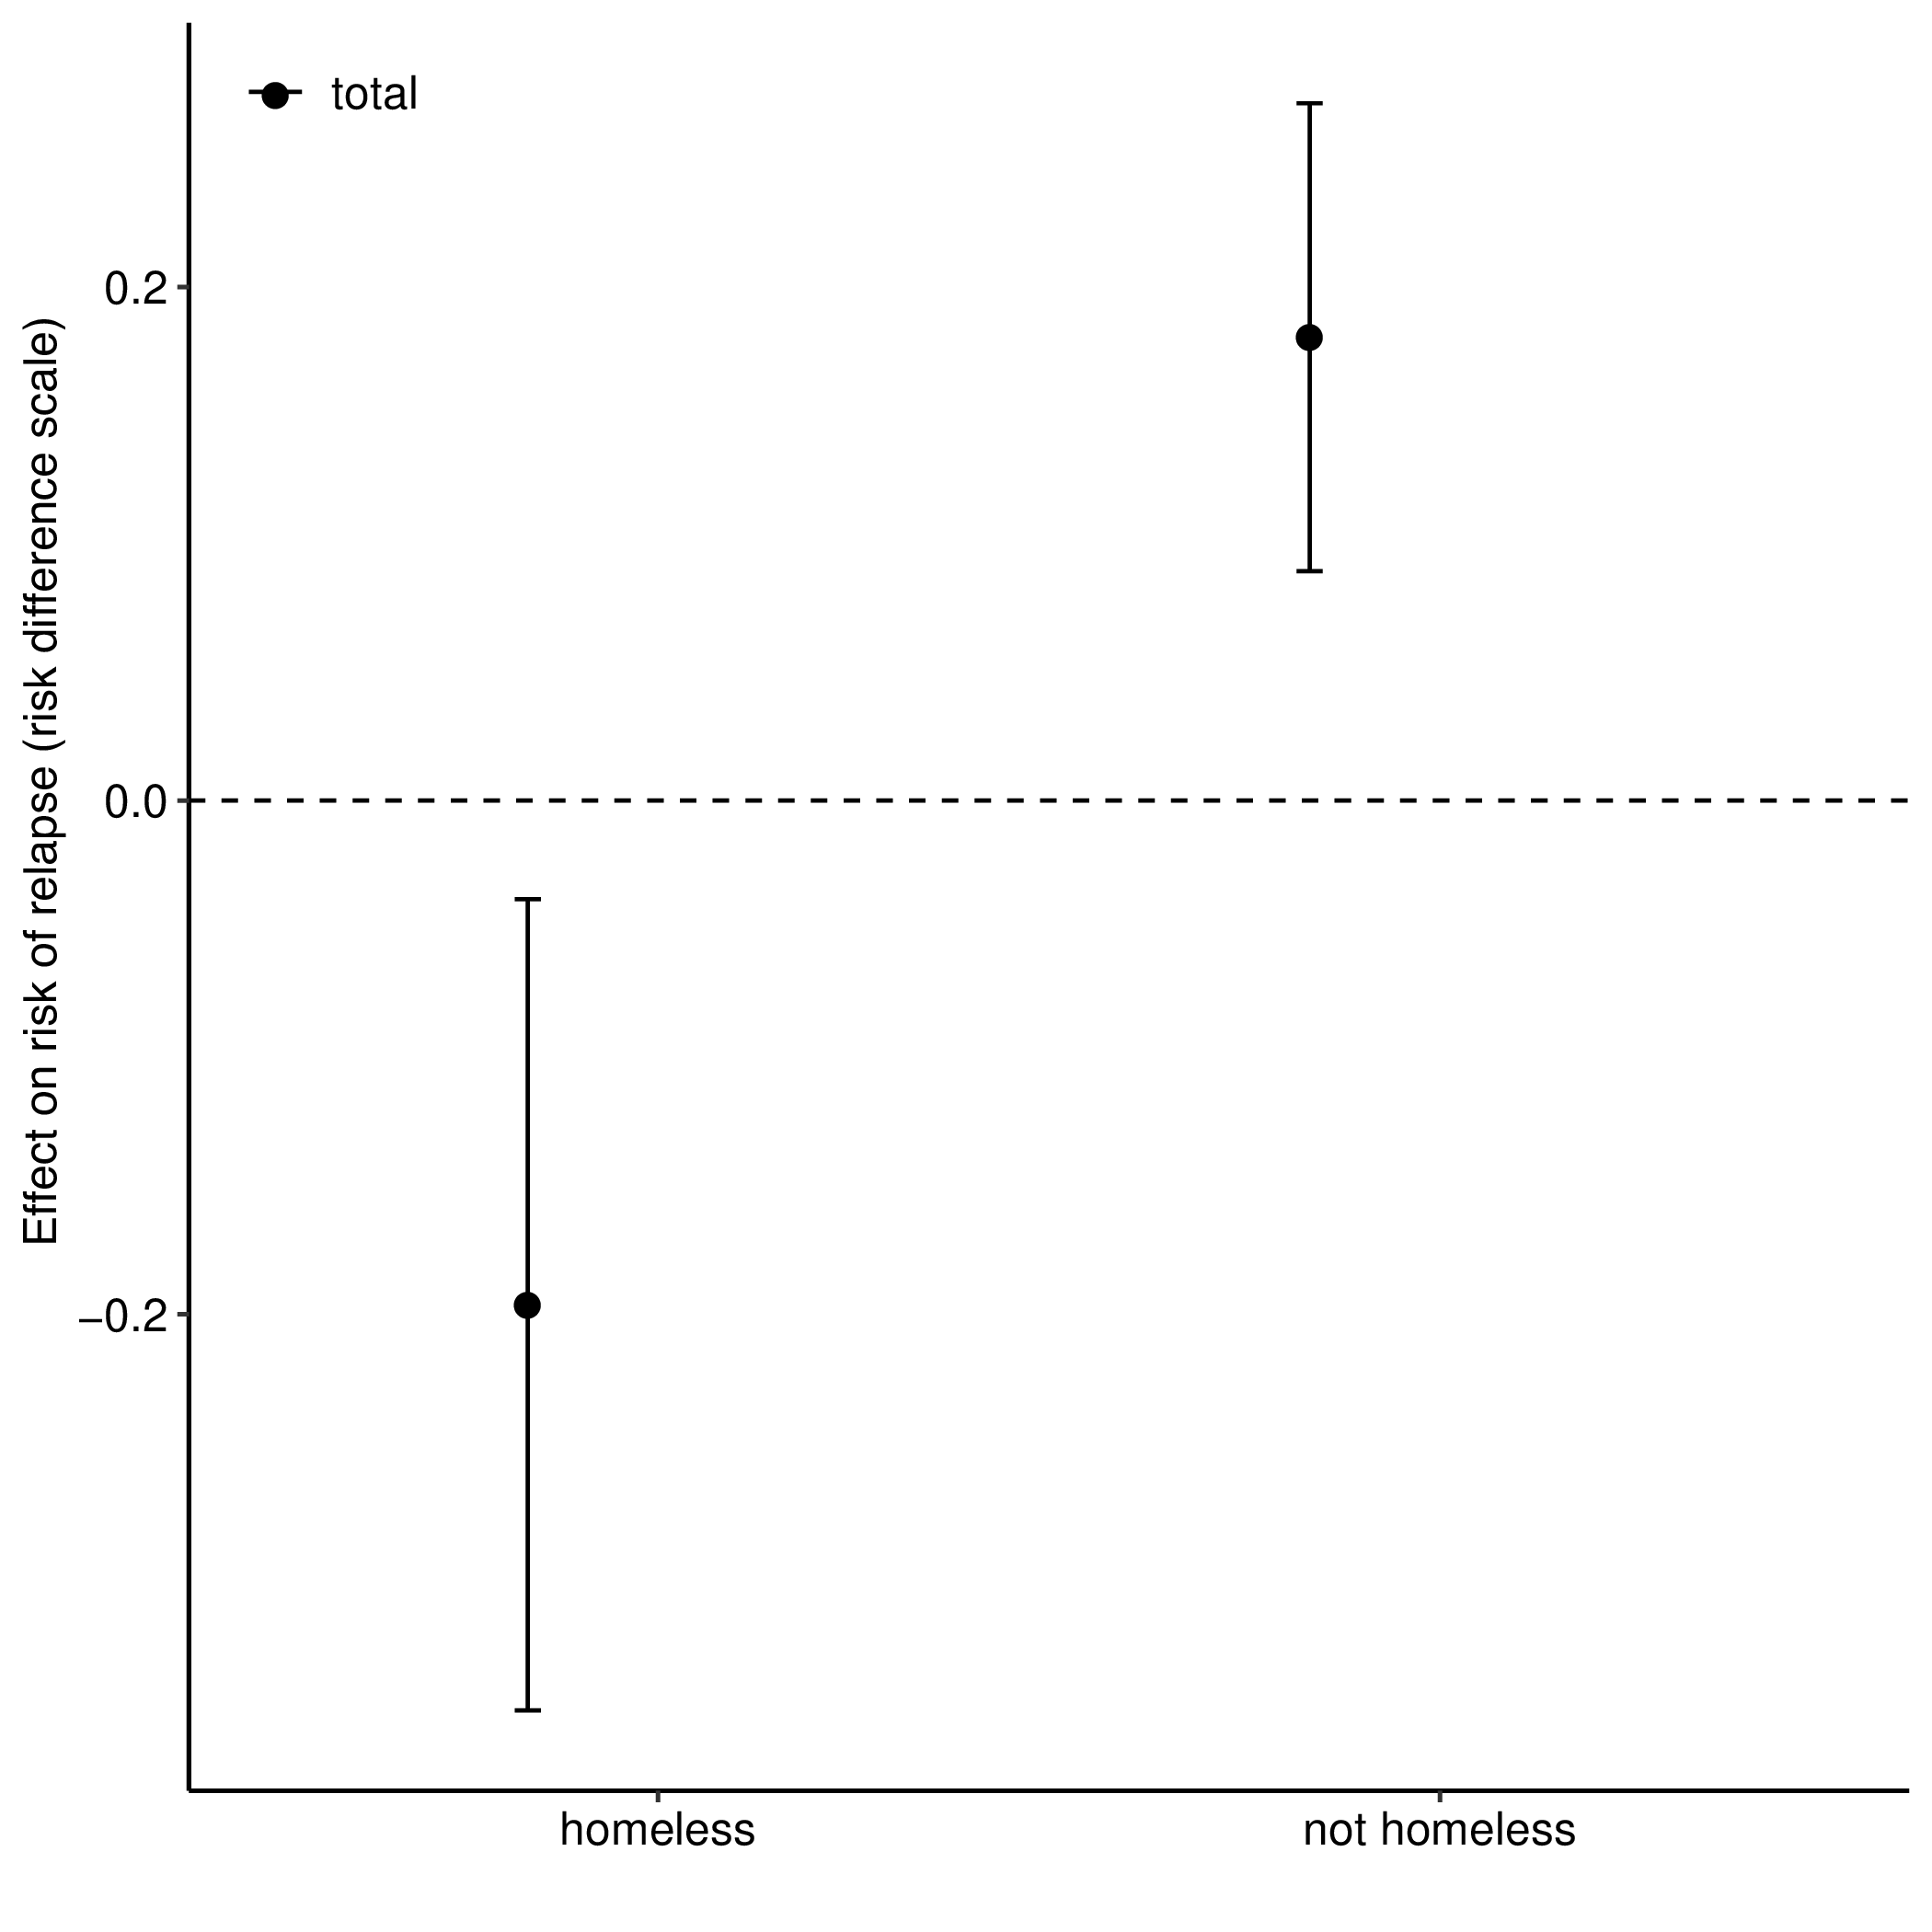
\includegraphics[width=0.75\linewidth]{/home/runner/work/ser2021_mediation_workshop/ser2021_mediation_workshop/img/tmleesttotal} 

}

\end{figure}

\hypertarget{getting-specific-about-the-question}{%
\subsection{Getting specific about the question}\label{getting-specific-about-the-question}}

To what extent does the indirect effect through mediators of adherence, pain, and
depressive symptoms explain the differences in treatment effects on OUD relapse
for homeless and nonhomeless individuals?

\hypertarget{what-estimand-do-we-want}{%
\subsubsection*{What estimand do we want?}\label{what-estimand-do-we-want}}


\begin{itemize}
\tightlist
\item
  Can we set \(M=m\) (i.e., same value) for everyone?
\item
  Are we interested in estimating indirect effects?
\end{itemize}

\(\rightarrow\) So, \emph{not} controlled direct effect.

\begin{itemize}
\tightlist
\item
  Do we have an intermediate confounder?
\item
  Yes, and it's important.
\end{itemize}

\(\rightarrow\) So, \emph{not} natural (in)direct effects.

\begin{itemize}
\tightlist
\item
  So, we're left with the interventional direct and indirect effects.
\item
  Do we want to estimate the path through treatment initiation (\(Z\))?
\item
  Yes, so, \emph{not} the conditional versions of these effects.
\item
  Estimands:

  \begin{itemize}
  \tightlist
  \item
    Direct effect: \(\E(Y_{1,G_0} - Y_{0,G_0})\)
  \item
    Indirect effect: \(\E(Y_{1,G_1} - Y_{1,G_0})\)
  \end{itemize}
\item
  Here \(G_a\) is a draw from the distribution of \(M_a\mid W\).
\item
  Need to incorporate multiple and continuous mediators
\end{itemize}

\hypertarget{what-if-the-positivity-assumption-paamid-w0-violated}{%
\subsubsection*{\texorpdfstring{What if the positivity assumption \(\P(A=a\mid W)>0\) violated?}{What if the positivity assumption \textbackslash P(A=a\textbackslash mid W)\textgreater0 violated?}}\label{what-if-the-positivity-assumption-paamid-w0-violated}}


\(\rightarrow\) Can't identify or estimate any of the above effects

\begin{itemize}
\tightlist
\item
  But we can estimate the effect of some stochastic interventions, e.g., IPSIs
\item
  Tradeoff between feasibility and interpretation
\end{itemize}

\hypertarget{what-if-the-exposure-variable-is-continuous}{%
\subsubsection*{What if the exposure variable is continuous?}\label{what-if-the-exposure-variable-is-continuous}}


\(\rightarrow\) All the above effects are defined for binary exposures

\begin{itemize}
\tightlist
\item
  But we can estimate the effect of some stochastic interventions
\item
  Work in progress (including upcoming R software)
\end{itemize}

\hypertarget{preliminaries-on-semiparametric-estimation}{%
\chapter{Preliminaries on semiparametric estimation}\label{preliminaries-on-semiparametric-estimation}}

\hypertarget{from-causal-to-statistical-quantities}{%
\section{From causal to statistical quantities}\label{from-causal-to-statistical-quantities}}

\begin{itemize}
\tightlist
\item
  We have arrived at identification formulas that express quantities that we
  care about in terms of observable quantities
\item
  That is, these formulas express what would have happened in hypothetical worlds in terms of quantities observable in this world
\item
  This required \textbf{causal assumptions}

  \begin{itemize}
  \tightlist
  \item
    Many of these assumptions are empirically unverifiable
  \item
    We saw an example where we could relax the cross-world assumption, at the
    cost of changing the parameter interpretation
  \item
    and where we could relax the positivity assumption, also at the cost of
    changing the parameter interpretation
  \end{itemize}
\item
  We are now ready to tackle the estimation problem, i.e., how do we best learn the value of quantities that are observable?
\item
  The resulting estimation problem can be tackled using \textbf{statistical
  assumptions} of various degrees of strength

  \begin{itemize}
  \tightlist
  \item
    Most of these assumptions are verifiable (e.g., a linear model)
  \item
    Thus, most are unnecessary (except for convenience)
  \item
    We have worked hard to try to satisfy the required causal assumptions
  \item
    This is not the time to introcuce unnecessary statistical assumptions
  \item
    The estimation approach we will introduce reduces reliance on these statistical
    assumptions
  \end{itemize}
\end{itemize}

\hypertarget{computing-identification-formulas-if-you-know-the-true-distribution}{%
\subsection{Computing identification formulas if you know the true distribution}\label{computing-identification-formulas-if-you-know-the-true-distribution}}

\begin{itemize}
\item
  The mediation parameters that we consider can be
  seen as a function of the joint probability distribution of \(O=(W,A,Z,M,Y)\)
\item
  For example, under identifiability assumptions the natural direct effect is
  equal to
  \begin{equation*}
    \psi(\P) =  \E[\color{Goldenrod}{\E\{\color{ForestGreen}{\{E(Y \mid A=1, M, W) - \E(Y \mid A=0, M, W)}\mid A=0,W\}}]
  \end{equation*}
\item
  The notation \(\psi(\P)\) implies that the parameter is a function of \(\P\)
\item
  This means that we can compute it for any distribution \(\P\)
\item
  For example, if we know the true \(\P(W,A,M,Y)\), we can comnpute the true value
  of the parameter by:

  \begin{itemize}
  \tightlist
  \item
    Computing the conditional expectation \(\E(Y\mid A=1,M=m,W=w)\) for all
    values \((m,w)\)
  \item
    Computing the conditional expectation \(\E(Y\mid A=0,M=m,W=w)\) for all
    values \((m,w)\)
  \item
    Computing the probability \(\P(M=m\mid A=0,W=w)\) for all values \((m,w)\)
  \item
    Compute
    \begin{align*}
    \color{Goldenrod}{\E\{}&\color{ForestGreen}{\E(Y \mid A=1, M, W) - \E(Y \mid A=0, M, W)}\color{Goldenrod}{\mid A=0,W\}} =\\
    &\color{Goldenrod}{\sum_m\color{ForestGreen}{\{\E(Y \mid A=1, m, w) - \E(Y \mid A=0, m, w)\}}\P(M=m, A=0, W=w)}
    \end{align*}
  \item
    Computing the probability \(\P(W=w)\) for all values \(w\)
  \item
    Computing the mean over all values \(w\)
  \end{itemize}
\end{itemize}

\hypertarget{estimating-identification-formulas}{%
\subsection{Estimating identification formulas}\label{estimating-identification-formulas}}

The above is how you would compute the \emph{true value} \textbf{if you know} the true
distribution \(\P\)

\begin{itemize}
\tightlist
\item
  This is exactly what we did in our R examples before
\item
  But we can use the same logic for estimation:

  \begin{itemize}
  \tightlist
  \item
    Fit a regression to estimate, say \(\hat\E(Y\mid A=1,M=m,W=w)\)
  \item
    Fit a regression to estimate, say \(\hat\E(Y\mid A=0,M=m,W=w)\)
  \item
    Fit a regression to estimate, say \(\hat\P(M=m\mid A=0,W=w)\)
  \item
    Estimate \(\P(W=w)\) with the empirical distribution
  \item
    Evaluate
    \begin{equation*}
      \psi(\hat\P) =  \hat\E[\hat\E\{\hat\E(Y \mid A=1, M, W) -
      \hat\E(Y \mid A=0, M, W)\mid A=0,W\}]
    \end{equation*}
  \end{itemize}
\item
  This is known as the g-computation estimator
\end{itemize}

\hypertarget{weighted-estimator-akin-to-ipw}{%
\subsection{Weighted estimator (akin to IPW)}\label{weighted-estimator-akin-to-ipw}}

\begin{itemize}
\tightlist
\item
  An alternative expresion of the parameter functional (for the NDE) is given by
\end{itemize}

\[\E\bigg[\color{RoyalBlue}{\bigg\{ \frac{I(A=1)}{\P(A=1\mid W)}\frac{\P(M\mid A=0,W)}{\P(M\mid A=1,W)} -
      \frac{I(A=0)}{\P(A=0\mid W)}\bigg\}} \times \color{Goldenrod}{Y}\bigg]\]

\begin{itemize}
\tightlist
\item
  Thus, you can also construct a weighted estimator as
\end{itemize}

\[\frac{1}{n}\sum_{i=1}^n\bigg[\color{RoyalBlue}{\bigg\{ \frac{I(A_i=1)}{\hat\P(A_i=1\mid W_i)}\frac{\hat\P(M_i\mid A_i=0,W_i)}{\hat\P(M_i\mid A_i=1,W_i)} -
      \frac{I(A_i=0)}{\hat\P(A_i=0\mid W_i)}\bigg\}} \times \color{Goldenrod}{Y}\bigg]\]

\hypertarget{how-can-g-estimation-and-weighted-estimation-be-implemented-in-practice}{%
\subsection{How can g-estimation and weighted estimation be implemented in practice?}\label{how-can-g-estimation-and-weighted-estimation-be-implemented-in-practice}}

\begin{itemize}
\tightlist
\item
  There are two possible ways to do g-computation estimation:

  \begin{itemize}
  \tightlist
  \item
    Using parametric models for the above regressions
  \item
    Using flexible data-adaptive regression (aka machine learning)
  \end{itemize}
\end{itemize}

\hypertarget{pros-and-cons-of-g-computation-and-weighting-parametric-models}{%
\subsection{Pros and cons of g-computation and weighting parametric models}\label{pros-and-cons-of-g-computation-and-weighting-parametric-models}}

\begin{itemize}
\tightlist
\item
  Pros:

  \begin{itemize}
  \tightlist
  \item
    Easy to understand
  \item
    Ease of implementation (standard regression software)
  \item
    Can use the Delta method or the bootstrap for computation of standard errors
  \end{itemize}
\item
  Cons:

  \begin{itemize}
  \tightlist
  \item
    Unless \(W\) and \(M\) contain very few categorical variables, it is very easy
    to misspecify the models
  \item
    This can introduce sizable bias in the estimators
  \item
    This modelling assumptions have become less necessary in the presence of data-adaptive regression tools (a.k.a machine learning)
  \end{itemize}
\end{itemize}

\hypertarget{an-example-of-the-bias-of-a-g-computation-estimator-of-the-natural-direct-effect}{%
\subsection{An example of the bias of a g-computation estimator of the natural direct effect}\label{an-example-of-the-bias-of-a-g-computation-estimator-of-the-natural-direct-effect}}

\begin{itemize}
\tightlist
\item
  The following \passthrough{\lstinline!R!} chunk provides simulation code to exemplify the bias of a
  g-computation parametric estimator in a simple situation
\end{itemize}

\begin{lstlisting}[language=R]
mean_y <- function(m, a, w) abs(w) + a * m
mean_m <- function(a, w) plogis(w^2 - a)
pscore <- function(w) plogis(1 - abs(w))
\end{lstlisting}

\begin{itemize}
\tightlist
\item
  This yields a true NDE value of 0.58048
\end{itemize}

\begin{lstlisting}[language=R]
w_big <- runif(1e6, -1, 1)
trueval <- mean((mean_y(1, 1, w_big) - mean_y(1, 0, w_big)) *
  mean_m(0, w_big) + (mean_y(0, 1, w_big) - mean_y(0, 0, w_big)) *
    (1 - mean_m(0, w_big)))
print(trueval)
#> [1] 0.58062
\end{lstlisting}

\begin{itemize}
\tightlist
\item
  Let's perform a simulation where we draw 1000 datasets from the above
  distribution, and compute a g-computation estimator based on
\end{itemize}

\begin{lstlisting}[language=R]
gcomp <- function(y, m, a, w) {
  lm_y <- lm(y ~ m + a + w)
  pred_y1 <- predict(lm_y, newdata = data.frame(a = 1, m = m, w = w))
  pred_y0 <- predict(lm_y, newdata = data.frame(a = 0, m = m, w = w))
  pseudo <- pred_y1 - pred_y0
  lm_pseudo <- lm(pseudo ~ a + w)
  pred_pseudo <- predict(lm_pseudo, newdata = data.frame(a = 0, w = w))
  estimate <- mean(pred_pseudo)
  return(estimate)
}
\end{lstlisting}

\begin{lstlisting}[language=R]
estimate <- lapply(seq_len(1000), function(iter) {
  n <- 1000
  w <- runif(n, -1, 1)
  a <- rbinom(n, 1, pscore(w))
  m <- rbinom(n, 1, mean_m(a, w))
  y <- rnorm(n, mean_y(m, a, w))
  est <- gcomp(y, m, a, w)
  return(est)
})
estimate <- do.call(c, estimate)

hist(estimate)
abline(v = trueval, col = "red", lwd = 4)
\end{lstlisting}

\begin{center}\includegraphics[width=0.8\linewidth]{05-preliminaries-estimation_files/figure-latex/unnamed-chunk-5-1} \end{center}

\begin{itemize}
\tightlist
\item
  The bias also affects the confidence intervals:
\end{itemize}

\begin{lstlisting}[language=R]
cis <- cbind(
  estimate - qnorm(0.975) * sd(estimate),
  estimate + qnorm(0.975) * sd(estimate)
)

ord <- order(rowSums(cis))
lower <- cis[ord, 1]
upper <- cis[ord, 2]
curve(trueval + 0 * x,
  ylim = c(0, 1), xlim = c(0, 1001), lwd = 2, lty = 3, xaxt = "n",
  xlab = "", ylab = "Confidence interval", cex.axis = 1.2, cex.lab = 1.2
)
for (i in 1:1000) {
  clr <- rgb(0.5, 0, 0.75, 0.5)
  if (upper[i] < trueval || lower[i] > trueval) clr <- rgb(1, 0, 0, 1)
  points(rep(i, 2), c(lower[i], upper[i]), type = "l", lty = 1, col = clr)
}
text(450, 0.10, "n=1000 repetitions = 1000 ", cex = 1.2)
text(450, 0.01, paste0(
  "Coverage probability = ",
  mean(lower < trueval & trueval < upper), "%"
), cex = 1.2)
\end{lstlisting}

\begin{center}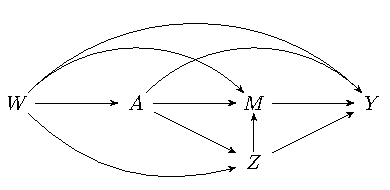
\includegraphics[width=0.8\linewidth]{05-preliminaries-estimation_files/figure-latex/unnamed-chunk-6-1} \end{center}

\hypertarget{pros-and-cons-of-g-computation-or-weighting-with-data-adaptive-regression}{%
\subsection{Pros and cons of g-computation or weighting with data-adaptive regression}\label{pros-and-cons-of-g-computation-or-weighting-with-data-adaptive-regression}}

\begin{itemize}
\tightlist
\item
  Pros:

  \begin{itemize}
  \tightlist
  \item
    Easy to understand
  \item
    Alleviate model-misspecification bias
  \end{itemize}
\item
  Cons:

  \begin{itemize}
  \tightlist
  \item
    Might be harder to implement depending on the regression procedures used
  \item
    No general approaches for computation of standard errors and confidence
    intervals
  \item
    For example, the bootstrap is not guaranteed to work, and it is known to
    fail in some cases
  \end{itemize}
\end{itemize}

\hypertarget{semiparametric-estimation}{%
\section{Semiparametric estimation}\label{semiparametric-estimation}}

\begin{itemize}
\tightlist
\item
  Intuitively, it offers a way to use data-adaptive regression to

  \begin{itemize}
  \tightlist
  \item
    avoid model misspecification bias,
  \item
    endow the estimators with additional robustness (e.g., double robustness), while
  \item
    allowing the computation of correct standard errors and confidence intervals
  \end{itemize}
\item
  This can be achieved by adding a bias correction factor the the g-computation
  as follows:
  \begin{equation*}
    \psi(\hat \P) + \frac{1}{n}\sum_{i=1}^n D(O_i)
  \end{equation*}
  for some function \(D(O_i)\) of the data
\item
  The function \(D(O)\) is called \emph{the efficient influence function} (EIF)
\item
  The EIF must be found on a case-by-case basis for each parameter \(\psi(\P)\)
\item
  For example, for estimating the standardized mean \(\psi(\P)=\E[\E(Y\mid A=1, W)]\), we have
  \begin{equation*}
    D(O) = \frac{A}{\hat \P(A=1\mid W)}[Y - \hat\E(Y\mid A=1, W)] +
    \hat\E(Y\mid A=1, W) - \psi(\hat\P)
  \end{equation*}
\item
  The EIF is found by using a distributional analogue of a Taylor expansion
\item
  In this workshop we will omit the specific form of \(D(O)\) for
  some of the parameters that we use
\item
  But the estimators we discuss and implement in the R packages will be based on
  these EIFs
\item
  And the specific form of the EIF may be found in papers in the references
\end{itemize}

Note: the bias correction above may have an additional problem of
returning parameter estimates outside of natural bounds. E.g.,
probabilities greater than one. A solution to this (not discussed in
this workshop but implemented in some of the R packages) is targeted
minimum loss based estimation.

\hypertarget{using-the-eif-to-construct-an-estimator-the-case-of-the-natural-direct-effect}{%
\chapter{Using the EIF to construct an estimator: the case of the natural direct effect}\label{using-the-eif-to-construct-an-estimator-the-case-of-the-natural-direct-effect}}

\hypertarget{natural-direct-effect}{%
\section{Natural direct effect}\label{natural-direct-effect}}

Recall:

\begin{figure}

{\centering \includegraphics[width=0.8\linewidth]{06-estimation-natural-interventional_files/figure-latex/unnamed-chunk-1-1} 

}

\caption{Directed acyclic graph under *no intermediate confounders* of the mediator-outcome relation affected by treatment}\label{fig:unnamed-chunk-1}
\end{figure}

\begin{itemize}
\item
  Assuming a binary \(A\), we define the natural direct effect as: \[NDE = E(Y_{1,M_{0}} - Y_{0,M_{0}}),\]
\item
  and the natural indirect effect as: \[NIE = E(Y_{1,M_{1}} - Y_{1,M_{0}}).\]
\item
  The observed data is \(O=(W, A, M, Y)\)
\end{itemize}

This SCM is represented in the above DAG and the following causal models:
\begin{align*}
  W & = f_W(U_W)\\
  A & = f_A(W, U_A)\\
  M & = f_M(W, A, U_M)\\
  Y & = f_Y(W, A, M, U_Y),
\end{align*}
where \((U_W, U_A,U_M, U_Y)\) are exogenous random errors.

We assume
- \(A\) is a single binary randomized treatment (and thus \(A = f_A(U_A)\))
- \(M\) is a single binary mediator
- There are no restrictions on the distribution of \(W\) or \(Y\)

Recall that we need to assume the following to identify the above caual effects
from our observed data:

\begin{itemize}
\tightlist
\item
  \(A \indep Y_{a,m} \mid W\)
\item
  \(M \indep Y_{a,m} \mid W, A\)
\item
  \(A \indep M_a \mid W\)
\item
  \(M_0 \indep Y_{1,m} \mid W\)
\item
  and positivity assumptions
\end{itemize}

Then, the NDE is identified as
\begin{equation*}
    \psi(\P) =  \E[\E\{\E(Y \mid A=1, M, W) - \E(Y \mid A=0, M, W)\mid A=0,W\}]
  \end{equation*}

\hypertarget{the-efficient-influence-function-for-the-nde}{%
\subsection{The efficient influence function for the NDE}\label{the-efficient-influence-function-for-the-nde}}

\begin{itemize}
\tightlist
\item
  For illustration, we will first present how to construct an estimator of the
  NDE that uses the EIF ``by hand''
\item
  For other parameters, we will teach you how to use our packages \emph{medoutcon}
  and \emph{medshift}
\end{itemize}

First, we need to introduce some notation to describe the EIF for the NDE

\begin{itemize}
\item
  Let \(Q(M, W)\) denote \(\E(Y\mid A=1, M, W) - \E(Y\mid A=0, M, W)\)
\item
  We can now introduce the EIF:
  \begin{align*}
    D(O) &= \color{RoyalBlue}{\bigg\{ \frac{I(A=1)}{\P(A=1\mid W)}\frac{\P(M\mid A=0,W)}{\P(M\mid A=1,W)} -
      \frac{I(A=0)}{\P(A=0\mid W)}\bigg\}} \times \color{Goldenrod}{[Y-\E(Y\mid A,M,W)]}  \\
    &+ \color{RoyalBlue}{\frac{I(A=0)}{\P(A=0\mid W)}}\color{Goldenrod}{\big\{Q(M,W) - \E[Q(M,W) | W,A=0] \big\}}\\
    &+ \color{Goldenrod}{\E[Q(M,W) | W,A=0] - \psi(\P)}
  \end{align*}
\item
  In this EIF, you can recognize elements from the g-computation estimator and the weighted estimator:

  \begin{itemize}
  \tightlist
  \item
    \(Q(M, W)\) shows up in the g-computation estimator
  \item
    The weights in blue in the first part of the EIF are used in the weighted estimator
  \end{itemize}
\item
  Estimating \(\P(M\mid A, W)\) is a really hard problem when \(M\) is
  high-dimensional. But, since we have the ratio of these conditional
  densitities, we can reparamterize using Bayes rule to get something that is
  easier to compute:
\end{itemize}

\begin{equation*}
  \frac{\P(M\mid A=0,W)}{\P(M\mid A=1,W)} = \frac{\P(A = 0 \mid M, W) \P(A=1
  \mid W)}{\P(A = 1 \mid M, W)\P(A=0 \mid W)}.
\end{equation*}

Thus we can change the expression of the EIF a bit as follows. First, some more
notation that will be useful later:

\begin{itemize}
\tightlist
\item
  Let \(g(a\mid w)\) denote \(\P(A=a\mid W=w)\)
\item
  Let \(e(a\mid m, w)\) denote \(\P(A=a\mid M=m, W=w)\)
\item
  Let \(b(a, m, w)\) denote \(\E(Y\mid A=a, M=m, W=w)\)
\item
  The EIF is
\end{itemize}

\begin{align*}
    D(O) &= \color{RoyalBlue}{\bigg\{ \frac{I(A=1)}{g(0\mid W)}\frac{e(0\mid M,W)}{e(1\mid M,W)} -
      \frac{I(A=0)}{g(0\mid W)}\bigg\}} \times \color{Goldenrod}{[Y-b(A,M,W)]}  \\
    &+ \color{RoyalBlue}{\frac{I(A=0)}{g(0\mid W)}}\color{Goldenrod}{\big\{Q(M,W) - \E[Q(M,W) | W,A=0] \big\}}\\
    &+ \color{Goldenrod}{\E[Q(M,W) | W,A=0] - \psi(\P)}
\end{align*}

\hypertarget{how-to-compute-the-one-step-estimator-akin-to-augmented-ipw}{%
\subsection{How to compute the one-step estimator (akin to Augmented IPW)}\label{how-to-compute-the-one-step-estimator-akin-to-augmented-ipw}}

First we will generate some data:

\begin{lstlisting}[language=R]
mean_y <- function(m, a, w) abs(w) + a * m
mean_m <- function(a, w)plogis(w^2 - a)
pscore <- function(w) plogis(1 - abs(w))

w_big <- runif(1e6, -1, 1)
trueval <- mean((mean_y(1, 1, w_big) - mean_y(1, 0, w_big)) * mean_m(0, w_big)
                + (mean_y(0, 1, w_big) - mean_y(0, 0, w_big)) *
                  (1 - mean_m(0, w_big)))

n <- 1000
w <- runif(n, -1, 1)
a <- rbinom(n, 1, pscore(w))
m <- rbinom(n, 1, mean_m(a, w))
y <- rnorm(n, mean_y(m, a, w))
\end{lstlisting}

Recall that the one-step estimator is defined as the bias-corrected
g-computation estimator:
\begin{equation*}
  \psi(\hat \P) + \frac{1}{n}\sum_{i=1}^n D(O;\hat \P_i)
\end{equation*}

Can be computed in the following steps:

\begin{enumerate}
\def\labelenumi{\arabic{enumi}.}
\tightlist
\item
  Fit models for \(g(a\mid w)\), \(e(a\mid m, w)\), and \(b(a, m, w)\)

  \begin{itemize}
  \tightlist
  \item
    In this example we will use Generalized Additive Models for
    tractability
  \item
    In applied settings we recommend using an ensemble of data-adaptive
    regression algorithms, such as the Super Learner \citep{vdl2007super}
  \end{itemize}
\end{enumerate}

\begin{lstlisting}[language=R]
library(mgcv)
## fit model for E(Y | A, W)
b_fit <- gam(y ~ m:a + s(w, by = a))
## fit model for P(A = 1 | M, W)
e_fit <- gam(a ~ m + w + s(w, by = m), family = binomial)
## fit model for P(A = 1 | W)
g_fit <- gam(a ~ w, family = binomial)
\end{lstlisting}

\begin{enumerate}
\def\labelenumi{\arabic{enumi}.}
\setcounter{enumi}{1}
\tightlist
\item
  Compute predictions \(g(1\mid w)\), \(g(0\mid w)\), \(e(1\mid m, w)\),
  \(e(0\mid m, w)\),\(b(1, m, w)\), \(b(0, m, w)\), and \(b(a, m, w)\)
\end{enumerate}

\begin{lstlisting}[language=R]
## Compute P(A = 1 | W)
g1_pred <- predict(g_fit, type = 'response')
## Compute P(A = 0 | W)
g0_pred <- 1 - g1_pred
## Compute P(A = 1 | M, W)
e1_pred <- predict(e_fit, type = 'response')
## Compute P(A = 0 | M, W)
e0_pred <- 1 - e1_pred
## Compute E(Y | A = 1, M, W)
b1_pred <- predict(b_fit, newdata = data.frame(a = 1, m, w))
## Compute E(Y | A = 0, M, W)
b0_pred <- predict(b_fit, newdata = data.frame(a = 0, m, w))
## Compute E(Y | A, M, W)
b_pred  <- predict(b_fit)
\end{lstlisting}

\begin{enumerate}
\def\labelenumi{\arabic{enumi}.}
\setcounter{enumi}{2}
\tightlist
\item
  Compute \(Q(M, W)\), fit a model for \(\E[Q(M,W) | W,A]\), and predict at \(A=0\)
\end{enumerate}

\begin{lstlisting}[language=R]
## Compute Q(M, W)
pseudo <- b1_pred - b0_pred
## Fit model for E[Q(M, W) | A, W]
q_fit <- gam(pseudo ~ a + w + s(w, by = a))
## Compute E[Q(M, W) | A = 0, W]
q_pred <- predict(q_fit, newdata = data.frame(a = 0, w = w))
\end{lstlisting}

\begin{enumerate}
\def\labelenumi{\arabic{enumi}.}
\setcounter{enumi}{3}
\tightlist
\item
  Estimate the weights
  \begin{equation*}
    \color{RoyalBlue}{\bigg\{ \frac{I(A=1)}{g(0\mid W)}\frac{e(0\mid M,W)}{e(1\mid M,W)} -
     \frac{I(A=0)}{g(0\mid W)}\bigg\}}
    \end{equation*}
  using the above predictions:
\end{enumerate}

\begin{lstlisting}[language=R]
ip_weights <- a / g0_pred * e0_pred / e1_pred - (1 - a) / g0_pred
\end{lstlisting}

\begin{enumerate}
\def\labelenumi{\arabic{enumi}.}
\setcounter{enumi}{4}
\tightlist
\item
  Compute the uncentered EIF:
\end{enumerate}

\begin{lstlisting}[language=R]
eif <- ip_weights * (y - b_pred) + (1 - a) / g0_pred * (pseudo - q_pred) +
  q_pred
\end{lstlisting}

\begin{enumerate}
\def\labelenumi{\arabic{enumi}.}
\setcounter{enumi}{5}
\tightlist
\item
  The one step estimator is the mean of the uncentered EIF
\end{enumerate}

\begin{lstlisting}[language=R]

## One-step estimator
mean(eif)
#> [1] 0.55085
\end{lstlisting}

\hypertarget{performance-of-the-one-step-estimator-in-a-small-simulation-study}{%
\subsection{Performance of the one-step estimator in a small simulation study}\label{performance-of-the-one-step-estimator-in-a-small-simulation-study}}

First, we create a wrapper around the estimator

\begin{lstlisting}[language=R]
one_step <- function(y, m, a, w) {
  b_fit <- gam(y ~ m:a + s(w, by = a))
  e_fit <- gam(a ~ m + w + s(w, by = m), family = binomial)
  g_fit <- gam(a ~ w, family = binomial)
  g1_pred <- predict(g_fit, type = 'response')
  g0_pred <- 1 - g1_pred
  e1_pred <- predict(e_fit, type = 'response')
  e0_pred <- 1 - e1_pred
  b1_pred <- predict(b_fit, newdata = data.frame(a = 1, m, w),
                 type = 'response')
  b0_pred <- predict(b_fit, newdata = data.frame(a = 0, m, w),
                     type = 'response')
  b_pred  <- predict(b_fit, type = 'response')
  pseudo <- b1_pred - b0_pred
  q_fit <- gam(pseudo ~ a + w + s(w, by = a))
  q_pred <- predict(q_fit, newdata = data.frame(a = 0, w = w))
  ip_weights <- a / g0_pred * e0_pred / e1_pred - (1 - a) / g0_pred
  eif <- ip_weights * (y - b_pred) + (1 - a) / g0_pred *
    (pseudo - q_pred) + q_pred
  return(mean(eif))
}
\end{lstlisting}

Let us first examine the bias

\begin{itemize}
\tightlist
\item
  The true value is:
\end{itemize}

\begin{lstlisting}[language=R]
w_big <- runif(1e6, -1, 1)
trueval <- mean((mean_y(1, 1, w_big) - mean_y(1, 0, w_big)) * mean_m(0, w_big) +
  (mean_y(0, 1, w_big) - mean_y(0, 0, w_big)) * (1 - mean_m(0, w_big)))
print(trueval)
#> [1] 0.58061
\end{lstlisting}

\begin{itemize}
\tightlist
\item
  Bias simulation
\end{itemize}

\begin{lstlisting}[language=R]
estimate <- lapply(seq_len(1000), function(iter) {
  n <- 1000
  w <- runif(n, -1, 1)
  a <- rbinom(n, 1, pscore(w))
  m <- rbinom(n, 1, mean_m(a, w))
  y <- rnorm(n, mean_y(m, a, w))
  estimate <- one_step(y, m, a, w)
  return(estimate)
})
estimate <- do.call(c, estimate)

hist(estimate)
abline(v = trueval, col = "red", lwd = 4)
\end{lstlisting}

\begin{center}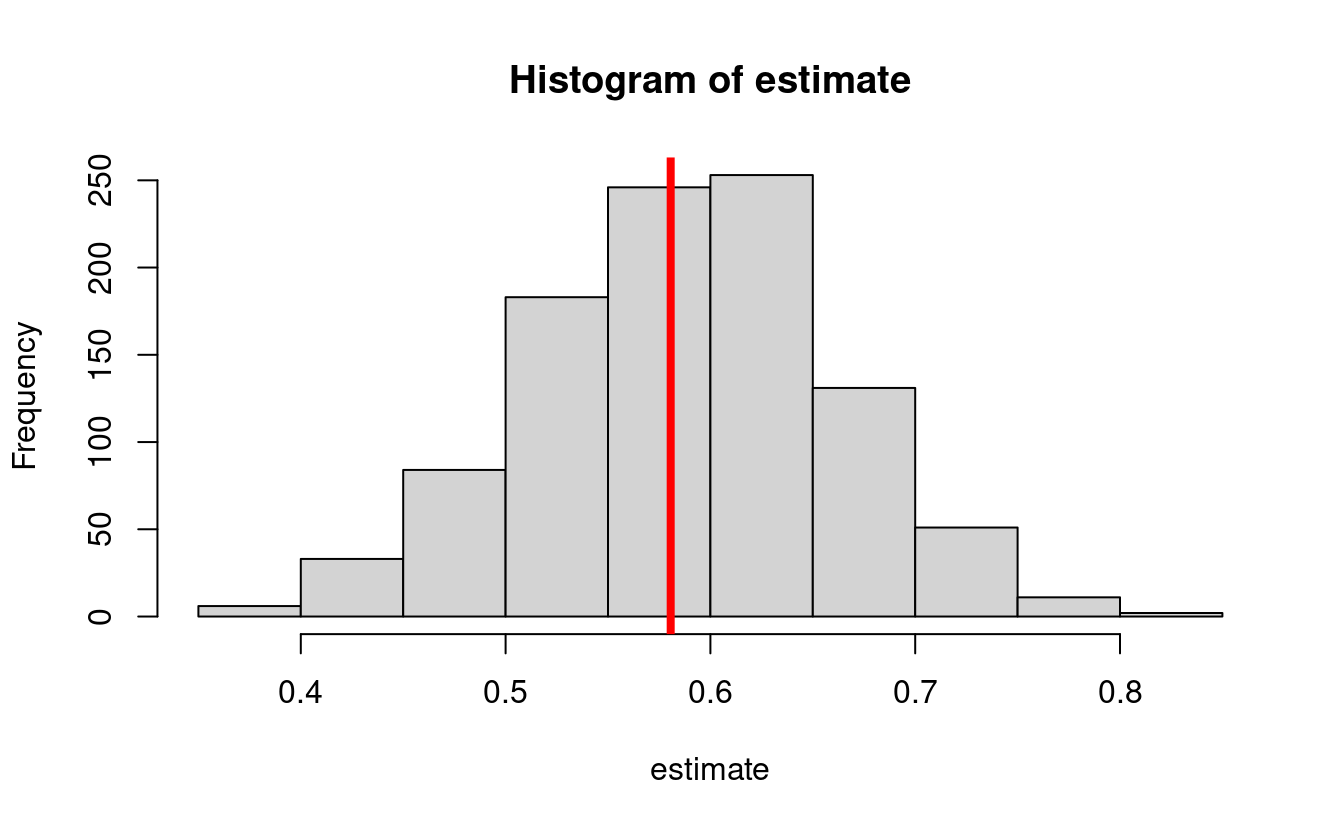
\includegraphics[width=0.8\linewidth]{06-estimation-natural-interventional_files/figure-latex/unnamed-chunk-11-1} \end{center}

\begin{itemize}
\tightlist
\item
  And now the confidence intervals:
\end{itemize}

\begin{lstlisting}[language=R]
cis <- cbind(
  estimate - qnorm(0.975) * sd(estimate),
  estimate + qnorm(0.975) * sd(estimate)
)

ord <- order(rowSums(cis))
lower <- cis[ord, 1]
upper <- cis[ord, 2]
curve(trueval + 0 * x,
  ylim = c(0, 1), xlim = c(0, 1001), lwd = 2, lty = 3, xaxt = "n",
  xlab = "", ylab = "Confidence interval", cex.axis = 1.2, cex.lab = 1.2
)
for (i in 1:1000) {
  clr <- rgb(0.5, 0, 0.75, 0.5)
  if (upper[i] < trueval || lower[i] > trueval) clr <- rgb(1, 0, 0, 1)
  points(rep(i, 2), c(lower[i], upper[i]), type = "l", lty = 1, col = clr)
}
text(450, 0.10, "n=1000 repetitions = 1000 ", cex = 1.2)
text(450, 0.01, paste0(
  "Coverage probability = ",
  mean(lower < trueval & trueval < upper), "%"
), cex = 1.2)
\end{lstlisting}

\begin{center}\includegraphics[width=0.8\linewidth]{06-estimation-natural-interventional_files/figure-latex/unnamed-chunk-12-1} \end{center}

\hypertarget{a-note-about-targeted-minimum-loss-based-estimation-tmle}{%
\subsection{A note about targeted minimum loss-based estimation (TMLE)}\label{a-note-about-targeted-minimum-loss-based-estimation-tmle}}

\begin{itemize}
\tightlist
\item
  The above estimator is great because it allows us to use data-adaptive regression to avoid bias, while allowing the computation of correct standard errors
\item
  This estimator has one problem:

  \begin{itemize}
  \tightlist
  \item
    It can yield answers outside of the bounds of the parameter space
  \item
    E.g., if \(Y\) is binary, it could yield direct and indirect effects outside of \([-1,1]\)
  \item
    To solve this, you can compute a TMLE instead (implemented in the R packages, coming up)
  \end{itemize}
\end{itemize}

\hypertarget{a-note-about-cross-fitting}{%
\subsection{A note about cross-fitting}\label{a-note-about-cross-fitting}}

\begin{itemize}
\tightlist
\item
  When using data-adaptive regression estimators, it is recommended to use cross-fitted estimators
\item
  Cross-fitting is similar to cross-validation:

  \begin{itemize}
  \tightlist
  \item
    Randomly split the sample into K (e.g., K=10) subsets of equal size
  \item
    For each of the 9/10ths of the sample, fit the regression models
  \item
    Use the out-of-sample fit to predict in the remaining 1/10th of the sample
  \end{itemize}
\item
  Cross-fitting further reduces the bias of the estimators
\item
  Cross-fitting aids in guaranteeing the correctness of the standard errors and confidence intervals
\item
  Cross-fitting is implemented by default in the R packages that you will see next
\end{itemize}

\hypertarget{r-packages-for-estimation-of-the-causal-indirect-effects}{%
\chapter{\texorpdfstring{\texttt{R} packages for estimation of the causal (in)direct effects}{R packages for estimation of the causal (in)direct effects}}\label{r-packages-for-estimation-of-the-causal-indirect-effects}}

We'll now turn to working through a few examples of estimating the natural,
interventional, and stochastic direct and indirect effects. As our running
example, we'll a simple data set from an observational study of the relationship
between BMI and kids' behavior, freely distributed with the \href{https://CRAN.R-project.org/package=mma}{\passthrough{\lstinline!mma!} \passthrough{\lstinline!R!} package
on CRAN}. First, let's load the packages
we'll be using and set a seed; then, load this data set and take a quick look

\begin{lstlisting}[language=R]
library(tidyverse)
library(sl3)
library(medoutcon)
library(medshift)
library(mma)
set.seed(429153)
\end{lstlisting}

\begin{lstlisting}[language=R]
# load and examine data
data(weight_behavior)
dim(weight_behavior)
#> [1] 691  15

# drop missing values
weight_behavior <- weight_behavior %>%
  drop_na() %>%
  as_tibble()
weight_behavior
#> # A tibble: 567 x 15
#>     bmi   age sex   race  numpeople   car gotosch snack tvhours cmpthours
#>   <dbl> <dbl> <fct> <fct>     <int> <int> <fct>   <fct>   <dbl>     <dbl>
#> 1  18.2  12.2 F     OTHER         5     3 2       1           4         0
#> 2  22.8  12.8 M     OTHER         4     3 2       1           4         2
#> 3  25.6  12.1 M     OTHER         2     3 2       1           0         2
#> 4  15.1  12.3 M     OTHER         4     1 2       1           2         1
#> 5  23.0  11.8 M     OTHER         4     1 1       1           4         3
#> # ... with 562 more rows, and 5 more variables: cellhours <dbl>, sports <fct>,
#> #   exercises <int>, sweat <int>, overweigh <dbl>
\end{lstlisting}

The documentation for the data set describes it as a ``database obtained from the
Louisiana State University Health Sciences Center, New Orleans, by Dr.~Richard
Scribner. He explored the relationship between BMI and kids' behavior through a
survey at children, teachers and parents in Grenada in 2014. This data set
includes 691 observations and 15 variables.'' Note that the data set contained
several observations with missing values, which we removed above to simplify the
demonstration of our analytic methods. In practice, we recommend instead using
appropriate corrections (e.g., imputation, inverse weighting) to fully take
advantage of the observed data.

Following the motivation of the original study, we focus on the causal effects
of participating in a sports team (\passthrough{\lstinline!sports!}) on the BMI of children (\passthrough{\lstinline!bmi!}),
taking into consideration several mediators (\passthrough{\lstinline!snack!}, \passthrough{\lstinline!exercises!}, \passthrough{\lstinline!overweigh!});
all other measured covariates are taken to be potential baseline confounders.

\hypertarget{medoutcon-natural-and-interventional-indirect-effects}{%
\section{\texorpdfstring{\texttt{medoutcon}: Natural and interventional (in)direct effects}{medoutcon: Natural and interventional (in)direct effects}}\label{medoutcon-natural-and-interventional-indirect-effects}}

The data on a single observational unit can be represented \(O = (W, A, M, Y)\),
with the data pooled across all participants denoted \(O_1, \ldots, O_n\), for a
of \(n\) i.i.d. observations of \(O\). Recall the DAG \protect\hyperlink{estimands}{from an earlier
chapter}, which represents the data-generating process:

\begin{figure}

{\centering \includegraphics[width=0.8\linewidth]{07-estimation-stochastic_files/figure-latex/unnamed-chunk-1-1} 

}

\caption{Directed acyclic graph under *no intermediate confounders* of the mediator-outcome relation affected by treatment}\label{fig:unnamed-chunk-1}
\end{figure}

\hypertarget{natural-indirect-effects}{%
\subsection{Natural (in)direct effects}\label{natural-indirect-effects}}

To start, we will consider estimation of the \emph{natural} direct and indirect effects,
which, we recall, are defined as follows
\begin{equation*}
  \E[Y_{1,M_1} - Y_{0,M_0}] = \underbrace{\E[Y_{\color{red}{1},\color{blue}{M_1}} -
    Y_{\color{red}{1},\color{blue}{M_0}}]}_{\text{natural indirect effect}} +
    \underbrace{\E[Y_{\color{blue}{1},\color{red}{M_0}} -
    Y_{\color{blue}{0},\color{red}{M_0}}]}_{\text{natural direct effect}}.
\end{equation*}

\begin{itemize}
\tightlist
\item
  Our \href{https://github.com/nhejazi/medoutcon}{\passthrough{\lstinline!medoutcon!} \passthrough{\lstinline!R!} package}
  \citep{hejazi2021medoutcon}, which accompanies \citet{diaz2020nonparametric}, implements
  one-step and TML estimators of both the natural and interventional (in)direct
  effects.
\item
  Both types of estimators are capable of accommodating flexible modeling
  strategies (e.g., ensemble machine learning) for the initial estimation of
  nuisance parameters.
\item
  The \passthrough{\lstinline!medoutcon!} \passthrough{\lstinline!R!} package uses cross-validation in initial estimation: this
  results in cross-validated (or ``cross-fitted'') one-step and TML estimators
  \citep{klaassen1987consistent, zheng2011cross, chernozhukov2018double}, which
  exhibit greater robustness than their non-sample-splitting analogs.
\item
  To this end, \passthrough{\lstinline!medoutcon!} integrates with the \passthrough{\lstinline!sl3!} \passthrough{\lstinline!R!} package, which is
  extensively documented in this \href{https://tlverse.org/tlverse-handbook/sl3}{book
  chapter} \citep{vdl2022targeted}.
\end{itemize}

\hypertarget{interlude-sl3-for-nuisance-parameter-estimation}{%
\subsection{\texorpdfstring{Interlude: \texttt{sl3} for nuisance parameter estimation}{Interlude: sl3 for nuisance parameter estimation}}\label{interlude-sl3-for-nuisance-parameter-estimation}}

\begin{itemize}
\tightlist
\item
  To fully take advantage of the one-step and TML estimators, we'd like to rely
  on flexible, data adaptive strategies for nuisance parameter estimation.
\item
  Doing so minimizes opportunities for model misspecification to compromise our
  analytic conclusions.
\item
  Choosing among the diversity of available machine learning algorithms can be
  challenging, so we recommend using the Super Learner algorithm for ensemble
  machine learning \citep{vdl2007super}, which is implemented in the \href{https://github.com/tlverse/sl3}{\passthrough{\lstinline!sl3!} R
  package} \citep{coyle2021sl3}.
\item
  Below, we demonstrate the construction of an ensemble learner based on a
  limited library of algorithms, including n intercept model, a main terms GLM,
  Lasso (\(\ell_1\)-penalized) regression, and random forest (\passthrough{\lstinline!ranger!}).
\end{itemize}

\begin{lstlisting}[language=R]
# instantiate learners
mean_lrnr <- Lrnr_mean$new()
fglm_lrnr <- Lrnr_glm_fast$new()
lasso_lrnr <- Lrnr_glmnet$new(alpha = 1, nfolds = 3)
rf_lrnr <- Lrnr_ranger$new(num.trees = 200)

# create learner library and instantiate super learner ensemble
lrnr_lib <- Stack$new(mean_lrnr, fglm_lrnr, lasso_lrnr, rf_lrnr)
sl_lrnr <- Lrnr_sl$new(learners = lrnr_lib, metalearner = Lrnr_nnls$new())
\end{lstlisting}

\begin{itemize}
\tightlist
\item
  Of course, there are many alternatives for learning algorithms to be included
  in such a modeling library. Feel free to explore!
\end{itemize}

\hypertarget{efficient-estimation-of-the-natural-indirect-effects}{%
\subsection{Efficient estimation of the natural (in)direct effects}\label{efficient-estimation-of-the-natural-indirect-effects}}

\begin{itemize}
\tightlist
\item
  Estimation of the natural direct and indirect effects requires estimation of a
  few nuisance parameters. Recall that these are

  \begin{itemize}
  \tightlist
  \item
    \(g(a\mid w)\), which denotes \(\P(A=a \mid W=w)\)
  \item
    \(h(a\mid m, w)\), which denotes \(\P(A=a \mid M=m, W=w)\)
  \item
    \(b(a, m, w)\), which denotes \(\E(Y \mid A=a, M=m, W=w)\)
  \end{itemize}
\item
  While we recommend the use of Super Learning, we opt to instead estimate all
  nuisance parameters with Lasso regression below (to save computational time).
\item
  Now, let's use the \passthrough{\lstinline!medoutcon()!} function to estimate the \emph{natural direct
  effect}:
\end{itemize}

\begin{lstlisting}[language=R]
# compute one-step estimate of the natural direct effect
nde_onestep <- medoutcon(
  W = weight_behavior[, c("age", "sex", "race", "tvhours")],
  A = (as.numeric(weight_behavior$sports) - 1),
  Z = NULL,
  M = weight_behavior[, c("snack", "exercises", "overweigh")],
  Y = weight_behavior$bmi,
  g_learners = lasso_lrnr,
  h_learners = lasso_lrnr,
  b_learners = lasso_lrnr,
  effect = "direct",
  estimator = "onestep",
  estimator_args = list(cv_folds = 5)
)
summary(nde_onestep)
#> # A tibble: 1 x 7
#>   lwr_ci param_est upr_ci var_est eif_mean estimator param         
#>    <dbl>     <dbl>  <dbl>   <dbl>    <dbl> <chr>     <chr>         
#> 1 -0.490   -0.0280  0.434  0.0555 2.84e-15 onestep   direct_natural
\end{lstlisting}

\begin{itemize}
\tightlist
\item
  We can similarly call \passthrough{\lstinline!medoutcon()!} to estimate the \emph{natural indirect effect}:
\end{itemize}

\begin{lstlisting}[language=R]
# compute one-step estimate of the natural indirect effect
nie_onestep <- medoutcon(
  W = weight_behavior[, c("age", "sex", "race", "tvhours")],
  A = (as.numeric(weight_behavior$sports) - 1),
  Z = NULL,
  M = weight_behavior[, c("snack", "exercises", "overweigh")],
  Y = weight_behavior$bmi,
  g_learners = lasso_lrnr,
  h_learners = lasso_lrnr,
  b_learners = lasso_lrnr,
  effect = "indirect",
  estimator = "onestep",
  estimator_args = list(cv_folds = 5)
)
summary(nie_onestep)
#> # A tibble: 1 x 7
#>   lwr_ci param_est upr_ci var_est eif_mean estimator param           
#>    <dbl>     <dbl>  <dbl>   <dbl>    <dbl> <chr>     <chr>           
#> 1  0.466      1.09   1.72   0.102 9.02e-16 onestep   indirect_natural
\end{lstlisting}

\begin{itemize}
\tightlist
\item
  From the above, we can conclude that the effect of participation on a sports
  team on BMI is primarily mediated by the variables \passthrough{\lstinline!snack!}, \passthrough{\lstinline!exercises!}, and
  \passthrough{\lstinline!overweigh!}, as the natural indirect effect is several times larger than the
  natural direct effect.
\item
  Note that we could have instead used the TML estimators, which have improved
  finite-sample performance, instead of the one-step estimators. Doing this is
  as simple as setting the \passthrough{\lstinline!estimator = "tmle"!} in the relevant argument.
\end{itemize}

\hypertarget{interventional-indirect-effects-1}{%
\subsection{Interventional (in)direct effects}\label{interventional-indirect-effects-1}}

Since our knowledge of the system under study is incomplete, we might worry that
one (or more) of the measured variables are not mediators, but, in fact,
intermediate confounders affected by treatment. While the natural (in)direct
effects are not identified in this setting, their interventional (in)direct
counterparts are, as we saw in an earlier section. Recall that both types of
effects are defined by static interventions on the treatment. The interventional
effects are distinguished by their use of a stochastic intervention on the
mediator to aid in their identification.

\begin{figure}
  
  {\centering 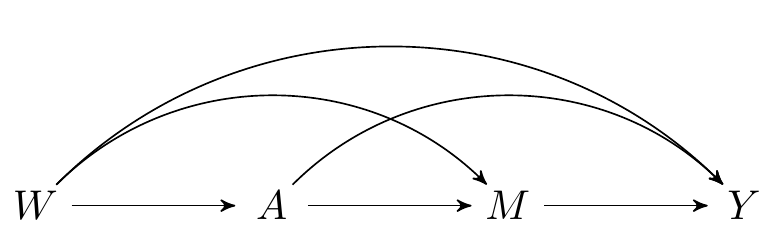
\includegraphics[width=0.8\linewidth]{07-estimation-stochastic_files/figure-latex/unnamed-chunk-2-1} 
  
  }
  
  \caption{Directed acyclic graph under intermediate confounders of the mediator-outcome relation affected by treatment}\label{fig:unnamed-chunk-2}
  \end{figure}

Recall that the interventional (in)direct effects are defined via the decomposition:
\begin{equation*}
\E[Y_{1,G_1} - Y_{0,G_0}] = \underbrace{\E[Y_{\color{red}{1},\color{blue}{G_1}} -
    Y_{\color{red}{1},\color{blue}{G_0}}]}_{\text{interventional indirect effect}} +
    \underbrace{\E[Y_{\color{blue}{1},\color{red}{G_0}} -
    Y_{\color{blue}{0},\color{red}{G_0}}]}_{\text{interventional direct effect}}
\end{equation*}

\begin{itemize}
\tightlist
\item
  In our data example, we'll consider the eating of snacks as a potential
  intermediate confounder, since one might reasonably hypothesize that
  participation on a sports team might subsequently affect snacking, which then
  could affect mediators like the amount of exercises and overweight status.
\item
  The interventional direct and indirect effects may also be easily estimated
  with the \href{https://github.com/nhejazi/medoutcon}{\passthrough{\lstinline!medoutcon!} \passthrough{\lstinline!R!} package}
  \citep{hejazi2021medoutcon}.
\item
  Just as for the natural (in)direct effects, \passthrough{\lstinline!medoutcon!} implements
  cross-validated one-step and TML estimators of the interventional effects.
\end{itemize}

\hypertarget{efficient-estimation-of-the-interventional-indirect-effects}{%
\subsection{Efficient estimation of the interventional (in)direct effects}\label{efficient-estimation-of-the-interventional-indirect-effects}}

\begin{itemize}
\tightlist
\item
  Estimation of these effects is more complex, so a few additional nuisance
  parameters arise when expressing the (more general) EIF for these effects:

  \begin{itemize}
  \tightlist
  \item
    \(q(z \mid a, w)\), the conditional density of the intermediate confounders,
    conditional only on treatment and baseline covariates;
  \item
    \(r(z \mid a, m, w)\), the conditional density of the intermediate
    confounders, conditional on mediators, treatment, and baseline covariates.
  \end{itemize}
\item
  To estimate the interventional effects, we only need to set the argument \passthrough{\lstinline!Z!}
  of \passthrough{\lstinline!medoutcon!} to a value other than \passthrough{\lstinline!NULL!}.
\item
  Note that the implementation in \passthrough{\lstinline!medoutcon!} is currently limited to settings
  with only binary intermediate confounders, i.e., \(Z \in \{0, 1\}\).
\item
  Let's use \passthrough{\lstinline!medoutcon()!} to estimate the \emph{interventional direct effect}:
\end{itemize}

\begin{lstlisting}[language=R]
# compute one-step estimate of the interventional direct effect
interv_de_onestep <- medoutcon(
  W = weight_behavior[, c("age", "sex", "race", "tvhours")],
  A = (as.numeric(weight_behavior$sports) - 1),
  Z = (as.numeric(weight_behavior$snack) - 1),
  M = weight_behavior[, c("exercises", "overweigh")],
  Y = weight_behavior$bmi,
  g_learners = lasso_lrnr,
  h_learners = lasso_lrnr,
  b_learners = lasso_lrnr,
  effect = "direct",
  estimator = "onestep",
  estimator_args = list(cv_folds = 5)
)
summary(interv_de_onestep)
#> # A tibble: 1 x 7
#>   lwr_ci param_est upr_ci var_est  eif_mean estimator param                
#>    <dbl>     <dbl>  <dbl>   <dbl>     <dbl> <chr>     <chr>                
#> 1 -0.476   -0.0107  0.454  0.0562 -9.93e-16 onestep   direct_interventional
\end{lstlisting}

\begin{itemize}
\tightlist
\item
  We can similarly estimate the \emph{interventional indirect effect}:
\end{itemize}

\begin{lstlisting}[language=R]
# compute one-step estimate of the interventional indirect effect
interv_ie_onestep <- medoutcon(
  W = weight_behavior[, c("age", "sex", "race", "tvhours")],
  A = (as.numeric(weight_behavior$sports) - 1),
  Z = (as.numeric(weight_behavior$snack) - 1),
  M = weight_behavior[, c("exercises", "overweigh")],
  Y = weight_behavior$bmi,
  g_learners = lasso_lrnr,
  h_learners = lasso_lrnr,
  b_learners = lasso_lrnr,
  effect = "indirect",
  estimator = "onestep",
  estimator_args = list(cv_folds = 5)
)
summary(interv_ie_onestep)
#> # A tibble: 1 x 7
#>   lwr_ci param_est upr_ci var_est eif_mean estimator param                  
#>    <dbl>     <dbl>  <dbl>   <dbl>    <dbl> <chr>     <chr>                  
#> 1  0.348     0.952   1.56  0.0950 3.15e-15 onestep   indirect_interventional
\end{lstlisting}

\begin{itemize}
\tightlist
\item
  From the above, we can conclude that the effect of participation on a sports
  team on BMI is largely through the interventional indirect effect (i.e.,
  through the pathways involving the mediating variables) rather than via its
  direct effect.
\item
  Just as before, we could have instead used the TML estimators, instead of the
  one-step estimators. Doing this is as simple as setting the
  \passthrough{\lstinline!estimator = "tmle"!} in the relevant argument.
\end{itemize}

\hypertarget{medshift-stochastic-indirect-effects}{%
\section{\texorpdfstring{\texttt{medshift}: Stochastic (in)direct effects}{medshift: Stochastic (in)direct effects}}\label{medshift-stochastic-indirect-effects}}

While the analyses using the natural and interventional effects have been
illuminating, we may also go beyond the restrictive static interventions
required to define these (in)direct effects. In fact, it may be more realistic
to consider interventions that do not directly force children to join athletic
teams, but instead motivate them to make their participation on such teams more
likely. Importantly, such interventions are often far more realistic and
actionable in real-world studies.

\hypertarget{formulating-the-stochastic-indirect-effects}{%
\subsection{Formulating the stochastic (in)direct effects}\label{formulating-the-stochastic-indirect-effects}}

\begin{itemize}
\tightlist
\item
  These more flexible intervention regimes are incompatible with (in)direct
  effect definitions based on decomposing the average treatment effect.
\item
  Instead, consider the decomposition of the population intervention effect
  (PIE) of a \emph{stochastic intervention} into direct and indirect effects
  \citep{diaz2020causal}:
  \begin{align*}
  \E[Y&_{A_\delta,M_{A_\delta}} - Y_{A,M_A}] = \\
  &\underbrace{\E[Y_{\color{red}{A_\delta},\color{blue}{M_{A_\delta}}} -
    Y_{\color{red}{A_\delta},\color{blue}{M}}]}_{\text{stochastic natural indirect effect}} +
    \underbrace{\E[Y_{\color{blue}{A_\delta},\color{red}{M}} -
    Y_{\color{blue}{A},\color{red}{M}}]}_{\text{stochastic natural direct effect}}
  \end{align*}
\item
  Recall from our discussion of the \protect\hyperlink{ipsi}{incremental propensity score
  interventions} \citep{kennedy2018nonparametric} that such stochastic
  interventions can compare the pre- and post-intervention odds of exposure:
  \begin{equation*}
  \delta = \frac{\text{odds}(A_\delta = 1\mid W=w)}
  {\text{odds}(A = 1\mid W=w)}.
  \end{equation*}
\item
  In our analysis, we will modulate the \emph{odds of participating in a sports
  team} by a fixed amount for each individual, setting, for example,
  \(\delta = 2\):
\end{itemize}

\begin{lstlisting}[language=R]
delta_shift_ipsi <- 2
\end{lstlisting}

\begin{itemize}
\tightlist
\item
  Such an intervention may be interpreted as the effect of a school program that
  motivates children to participate in sports teams.
\end{itemize}

\hypertarget{efficient-estimation-of-the-stochastic-indirect-effects}{%
\subsection{Efficient estimation of the stochastic (in)direct effects}\label{efficient-estimation-of-the-stochastic-indirect-effects}}

\begin{itemize}
\tightlist
\item
  The decomposition of the PIE into the direct and indirect effects leads to a
  common term \(\E[Y_{\color{red}{A_\delta},\color{blue}{M}}]\) involved in both
  the direct and indirect effect definitions. This term may be estimated via the
  \href{https://github.com/nhejazi/medshift}{\passthrough{\lstinline!medshift!} \passthrough{\lstinline!R!} package}
  \citep{hejazi2020medshift}.
\item
  For the direct effect, the remaining term is the
  \(\E[Y_{\color{blue}{A},\color{red}{M}}]\), which may be estimated by a simple
  mean in the observed data (i.e., no intervention).
\item
  For the indirect effect, the remaining term is the joint effect of stochastic
  interventions on both \(A\) and \(M\):
  \(\E[Y_{\color{red}{A_\delta},\color{blue}{M_{A_\delta}}}\).

  \begin{itemize}
  \tightlist
  \item
    For the case of an IPSI on binary \(A\), this may be estimated by the tools
    in the \href{https://github.com/ehkennedy/npcausal}{\passthrough{\lstinline!npcausal!} \passthrough{\lstinline!R!} package}.
  \item
    For the case of an MTP on continuous \(A\), this may be estimated by the tools
    in the \href{https://github.com/nhejazi/txshift}{\passthrough{\lstinline!txshift!} \passthrough{\lstinline!R!} package}
    \citep{hejazi2020txshift-rpkg, hejazi2020txshift-joss}.
  \end{itemize}
\item
  Like the implementation in \passthrough{\lstinline!medoutcon!}, the \passthrough{\lstinline!medshift!} package makes use of
  cross-validation in constructing initial estimates of nuisance parameters,
  resulting in more robust, cross-validated efficient estimators
  \citep{klaassen1987consistent, zheng2011cross, chernozhukov2018double}.
\item
  Now, we're ready to use the \passthrough{\lstinline!medshift!} function to estimate the decomposition
  term common to both the \emph{stochastic direct and indirect effects}:
\end{itemize}

\begin{lstlisting}[language=R]
# compute one-step estimate of the decomposition term of the (in)direct effects
stoch_decomp_onestep <- medshift(
  W = weight_behavior[, c("age", "sex", "race", "tvhours")],
  A = (as.numeric(weight_behavior$sports) - 1),
  Z = weight_behavior[, c("snack", "exercises", "overweigh")],
  Y = weight_behavior$bmi,
  delta = delta_shift_ipsi,
  g_learners = lasso_lrnr,
  e_learners = lasso_lrnr,
  m_learners = lasso_lrnr,
  estimator = "onestep",
  estimator_args = list(cv_folds = 5)
)
summary(stoch_decomp_onestep)
#>      lwr_ci   param_est      upr_ci   param_var    eif_mean   estimator 
#>   18.770026   19.103221   19.436415      0.0289 -1.7263e-15     onestep
\end{lstlisting}

\begin{itemize}
\tightlist
\item
  To estimate the stochastic direct effect, an extra step is necessary -- we
  must apply the delta method:
\end{itemize}

\begin{lstlisting}[language=R]
# convenience function to compute inference via delta method: EY1 - EY0
linear_contrast <- function(params, eifs, ci_level = 0.95) {
  # bounds for confidence interval
  ci_norm_bounds <- c(-1, 1) * abs(stats::qnorm(p = (1 - ci_level) / 2))
  param_est <- params[[1]] - params[[2]]
  eif <- eifs[[1]] - eifs[[2]]
  se_eif <- sqrt(var(eif) / length(eif))
  param_ci <- param_est + ci_norm_bounds * se_eif
  # parameter and inference
  out <- c(param_ci[1], param_est, param_ci[2])
  names(out) <- c("lwr_ci", "param_est", "upr_ci")
  return(out)
}
\end{lstlisting}

\begin{itemize}
\tightlist
\item
  Straightforward application of this procedure yields,
\end{itemize}

\begin{lstlisting}[language=R]
# parameter estimates and EIFs for components of direct effect
EY <- mean(weight_behavior$bmi)
eif_EY <- weight_behavior$bmi - EY
params_de <- list(stoch_decomp_onestep$theta, EY)
eifs_de <- list(stoch_decomp_onestep$theta, eif_EY)

# direct effect = EY - estimated quantity
de_est <- linear_contrast(params_de, eifs_de)
de_est
#>    lwr_ci param_est    upr_ci 
#> -0.347205 -0.023887  0.299430
\end{lstlisting}

\begin{itemize}
\tightlist
\item
  From the above, we can conclude that the effect of increasing the odds of
  participation on a sports team on BMI leads only to a relatively small direct
  effect.
\end{itemize}

  \bibliography{book.bib,packages.bib}

\backmatter
\printindex

\end{document}
